\begin{flushright} {\tiny {\color{gray} app\_elemental\_matrix.tex}} \end{flushright}

In what follows I compute the mass matrix for a variety of reference elements.
If you wish to use these in a code, do not forget to take the jacobian 
of the transformation/mapping into account. 

%---------------------------
\section{1d segments}

%.....................................
\subsection{Linear basis functions}

Let us start with the mass matrix (which we encountered in 
Section~\ref{sec:diff1D} -- although we leave the $\rho C_p$ term out, 
thereby implicitely assuming it is constant over the element!):
\begin{equation}
{\bm M}_e=\int_{\Omega_e} \vec{\bN}^T \vec{\bN} dV
= \int_{-1}^{+1} \vec{\bN}^T \vec{\bN} dr
\end{equation}
on the reference element, with 
\[
{\vec N}^T = 
\left(
\begin{array}{c}
\bN_1(r) \\ \bN_2(r)
\end{array}
\right)
=
\frac{1}{2}
\left(
\begin{array}{c}
1-r \\ 1+r
\end{array}
\right)
\]
We have 
\begin{eqnarray}
\int_{-1}^{+1} \bN_1(r) \bN_1(r)\; dr &=& 2/3 \nn\\ 
\int_{-1}^{+1} \bN_1(r) \bN_2(r)\; dr &=& 1/3 \nn\\
\int_{-1}^{+1} \bN_2(r) \bN_2(r)\; dr &=& 2/3 \nn
\end{eqnarray}
We then obtain 
\[
\boxed{
{\bm M}^e= \frac{1}{3} 
\left(
\begin{array}{cc}
2  & 1 \\
1 & 2
\end{array}
\right)}
\]
The lumped mass matrix is then
\begin{eqnarray}
\bar{\bm M}^e 
&=&
\frac{1}{3}
\left(
\begin{array}{cc}
2+1  & 0 \\
0 & 1+2
\end{array}
\right)
=
\left(
\begin{array}{cc}
1  & 0 \\
0 & 1
\end{array}
\right)
\end{eqnarray}

\begin{remark} 
The sum of all the terms in the mass matrix must be equal to 2. Proof: 
\begin{eqnarray}
\sum_{ij} M_{ij} 
&=&\sum_{ij} \int_{-1}^{+1} \bN_i \bN_j dr \nn\\
&=&\int_{-1}^{+1} (\bN_1\bN_1+\bN_1\bN_2+\bN_2\bN_1+\bN_2\bN_2) dr\nn\\
&=&\int_{-1}^{+1} [\bN_1(\bN_1+\bN_2)+\bN_2(\bN_1+\bN_2)]dr\nn\\
&=&\int_{-1}^{+1} (\bN_1 + \bN_2) dr\nn\\
&=& 2\nn
\end{eqnarray}
\end{remark}


%.....................................
\subsection{Quadratic basis functions}
There are now three nodes in the segment so that the mass matrix 
is now a $3\times3$ matrix. We have (see Section~\ref{sec:bf1}) 
\begin{equation}
{\vec \bN}^T(r) = 
\left(
\begin{array}{c}
\bN_1(r) \\ 
\bN_2(r) \\ 
\bN_3(r) 
\end{array}
\right)
=
\left(
\begin{array}{c}
\frac{1}{2} r (r-1) \\
1-r^2 \\
\frac{1}{2} r (r+1) 
\end{array}
\right)
\end{equation}
We then have to compute
\begin{eqnarray}
\int_{-1}^{+1} \bN_1(r) \bN_1(r) dr &=& \frac{8}{30}  = 0.26666 \nn\\
\int_{-1}^{+1} \bN_1(r) \bN_2(r) dr &=& \frac{4}{30}  =0.13333  \nn\\
\int_{-1}^{+1} \bN_1(r) \bN_3(r) dr &=& -\frac{2}{30} =-0.06666\nn\\ 
\int_{-1}^{+1} \bN_2(r) \bN_2(r) dr &=& \frac{16}{15} = 1.06666 \nn\\
\int_{-1}^{+1} \bN_2(r) \bN_3(r) dr &=& \frac{4}{30}  =0.13333 \nn\\
\int_{-1}^{+1} \bN_3(r) \bN_3(r) dr &=& \frac{8}{30} = 0.26666  \nn
\end{eqnarray}
and finally 
\begin{equation}
\boxed{
{\bm M}^e 
=\frac{1}{30}
\left(
\begin{array}{ccc}
8  & 4 & -2 \\
4  & 32 & 4 \\
-2 & 4 & 8
\end{array}
\right)
}
\end{equation}
The lumped mass matrix is then
\begin{eqnarray}
\bar{\bm M}^e 
&=&
\frac{1}{30}
\left(
\begin{array}{ccc}
8 + 4  -2 & 0 & 0\\
0 & 4 + 32 + 4 \\
0 & 0 & -2 + 4 + 8
\end{array}
\right) \nn\\
&=&
\frac{1}{30}
\left(
\begin{array}{ccc}
10 & 0 & 0\\
0 & 40 & 0\\
0 & 0 & 10 
\end{array}
\right) \nn\\
&=&
\frac{1}{3}
\left(
\begin{array}{ccc}
1 & 0 & 0\\
0 & 4 & 0\\
0 & 0 & 1 
\end{array}
\right) 
\end{eqnarray}
We can easily verify that
\[
\sum_{ij} M_{ij} = 2
\qquad
\qquad
\sum_{ij} \bar{M}_{ij} = 2
\]


%.....................................
\subsection{Cubic basis functions}
There are now four nodes in the segment so that the mass matrix 
is now a $4\times4$ matrix. We have (see Section~\ref{sec:bf3}) 
\begin{equation}
{\vec N}^T(r) = 
\left(
\begin{array}{c}
\bN_1(r) \\ 
\bN_2(r) \\ 
\bN_3(r) \\ 
\bN_4(r) 
\end{array}
\right)
=
\frac{1}{16}
\left(
\begin{array}{c}
 -1+  r+9r^2- 9r^3  \\ 
  9-27r-9r^2+27r^3  \\
  9+27r-9r^2-27r^3  \\
 -1-  r+9r^2+ 9r^3  
\end{array}
\right)
\end{equation}
leading to
\begin{eqnarray}
\int_{-1}^{+1} \bN_1(r) \bN_1(r) dr &=&  \frac{1}{256}\frac{4096}{105} \nn\\ 
\int_{-1}^{+1} \bN_1(r) \bN_2(r) dr &=&  \frac{1}{256}\frac{1056}{35} \nn\\
\int_{-1}^{+1} \bN_1(r) \bN_3(r) dr &=& -\frac{1}{256}\frac{384}{35} \nn\\
\int_{-1}^{+1} \bN_1(r) \bN_4(r) dr &=&  \frac{1}{256}\frac{608}{105} \nn\\
\int_{-1}^{+1} \bN_2(r) \bN_2(r) dr &=&  \frac{1}{256}\frac{6912}{35} \nn\\
\int_{-1}^{+1} \bN_2(r) \bN_3(r) dr &=& -\frac{1}{256}\frac{864}{35} \nn\\
\int_{-1}^{+1} \bN_2(r) \bN_4(r) dr &=& -\frac{1}{256}\frac{384}{35} \nn\\
\int_{-1}^{+1} \bN_3(r) \bN_3(r) dr &=&  \frac{1}{256}\frac{6912}{35}\nn\\
\int_{-1}^{+1} \bN_3(r) \bN_4(r) dr &=&  \frac{1}{256}\frac{1056}{35}\nn\\
\int_{-1}^{+1} \bN_4(r) \bN_4(r) dr &=&  \frac{1}{256}\frac{4096}{105}\nn
\end{eqnarray}
and finally 
\begin{equation}
\boxed{
{\bm M}^e 
=
\frac{1}{16}\frac{1}{105}
\left(
\begin{array}{cccc}
256 & 198 & -72  & 38  \\
198 & 1296 & -162 & -72 \\
-72 & -162 & 1296 & 198 \\
38 & -72 & 198 & 256
\end{array}
\right)}
\end{equation}
The lumped mass matrix is then
\begin{small}
\begin{eqnarray}
\bar{\bm M}^e 
&=&
\frac{1}{16}\frac{1}{105}
\left(
\begin{array}{cccc}
256 + 198 -72  +38 & 0 & 0 & 0  \\
0 & 198 + 1296  -162 -72 & 0 & 0\\
0 & 0 & -72 -162 + 1296 + 198 & 0\\
0 & 0 & 0 & 38 -72 + 198 + 256
\end{array}
\right) \nn\\
&=&
\frac{1}{16}\frac{1}{105}
\left(
\begin{array}{cccc}
420 & 0 & 0 & 0  \\
0 & 1260 & 0 & 0\\
0 & 0 & 1260 & 0\\
0 & 0 & 0 & 420
\end{array}
\right) \nn\\
&=&
\frac{1}{4}
\left(
\begin{array}{cccc}
1 & 0 & 0 & 0  \\
0 & 3 & 0 & 0\\
0 & 0 & 3 & 0\\
0 & 0 & 0 & 1
\end{array}
\right) \nn
\end{eqnarray}
\end{small}
We can easily verify that
\[
\sum_{ij} M_{ij} = 2
\qquad
\qquad
\sum_{ij} \bar{M}_{ij} = 2
\]


%.....................................
\subsection{Quartic basis functions}
There are now five nodes in the segment so that the mass matrix 
is a $5\times5$ matrix. We have (see Section~\ref{sec:bf4}) 
\begin{equation}
{\vec \bN}^T(r) = 
\left(
\begin{array}{c}
\bN_1(r) \\ 
\bN_2(r) \\ 
\bN_3(r) \\ 
\bN_4(r) \\ 
\bN_5(r) 
\end{array}
\right)
=
\frac{1}{6}
\left(
\begin{array}{c}
  r- r^2 -4r^3 +4r^4 \\
  -8r+16 r^2 +8r^3 -16 r^4  \\
6 -30r^2+24r^4   \\
  8r+16 r^2 -8r^3 -16 r^4  \\
  -r- r^2 +4r^3 +4r^4
\end{array}
\right)
\end{equation}
leading to
\begin{eqnarray}
\int_{-1}^{+1} \bN_1(r) \bN_1(r) dr &=& \frac{1}{36}\frac{1168}{315} \nn\\ 
\int_{-1}^{+1} \bN_1(r) \bN_2(r) dr &=& \frac{1}{36}\frac{1184}{315} \nn\\ 
\int_{-1}^{+1} \bN_1(r) \bN_3(r) dr &=&-\frac{1}{36}\frac{232}{105}  \nn\\ 
\int_{-1}^{+1} \bN_1(r) \bN_4(r) dr &=& \frac{1}{36}\frac{32}{45}    \nn\\ 
\int_{-1}^{+1} \bN_1(r) \bN_5(r) dr &=&-\frac{1}{36}\frac{116}{315}  \nn\\ 
\int_{-1}^{+1} \bN_2(r) \bN_2(r) dr &=& \frac{1}{36}\frac{1024}{45}  \nn\\ 
\int_{-1}^{+1} \bN_2(r) \bN_3(r) dr &=&-\frac{1}{36}\frac{512}{105}  \nn\\ 
\int_{-1}^{+1} \bN_2(r) \bN_4(r) dr &=& \frac{1}{36}\frac{1024}{315} \nn\\ 
\int_{-1}^{+1} \bN_2(r) \bN_5(r) dr &=& \frac{1}{36}\frac{32}{45}    \nn\\ 
\int_{-1}^{+1} \bN_3(r) \bN_3(r) dr &=& \frac{1}{36}\frac{832}{35}    \nn\\ 
\int_{-1}^{+1} \bN_3(r) \bN_4(r) dr &=& -\frac{1}{36}\frac{512}{105}    \nn\\ 
\int_{-1}^{+1} \bN_3(r) \bN_5(r) dr &=& -\frac{1}{36}\frac{232}{105}    \nn\\ 
\int_{-1}^{+1} \bN_4(r) \bN_4(r) dr &=& \frac{1}{36}\frac{1024}{45}    \nn\\ 
\int_{-1}^{+1} \bN_4(r) \bN_5(r) dr &=& \frac{1}{36}\frac{1184}{315}    \nn\\ 
\int_{-1}^{+1} \bN_5(r) \bN_5(r) dr &=& \frac{1}{36}\frac{1168}{315}    
\end{eqnarray}
and finally
\begin{equation}
\boxed{
{\bm M}^e
=\frac{1}{36}
\frac{1}{315}
\left(
\begin{array}{ccccc}
1168 & 1184 & -696 & 224 & -116 \\
1184 & 7168   & -1536  &  1024 &  224 \\
-696 & -1536 & 7488  & -1536  & -696  \\
224   & 1024 & -1536 & 7168 & 1184 \\
-116 & 224   & -696 & 1184 & 1168
\end{array}
\right)}
\end{equation}
The lumped mass matrix is then
\begin{eqnarray}
\bar{\bm M}^e 
&=&
=\frac{1}{36}
\frac{1}{315}
\left(
\begin{array}{ccccc}
1764 &0&0&0&0\\
0&8064 &0&0&0\\
0&0&3024 &0&0\\
0&0&0&8064 &0\\
0&0&0&0&1764 
\end{array}
\right)
=
\frac{1}{45}
\left(
\begin{array}{ccccc}
7 &0&0&0&0 \\
0&32 &0&0&0 \\
0&0&12  &0&0 \\
0&0&0&32   &0 \\
0&0&0&0&7      \\
\end{array}
\right) \nn
\end{eqnarray}
We can once again easily verify that
\[
\sum_{ij} M_{ij} = 2
\qquad
\qquad
\sum_{ij} \bar{M}_{ij} = 2
\]


Note that all the integrals above were done very conveniently 
with the WolframAlpha software/website\footnote{\url{https://www.wolframalpha.com/}}.
Example:

\begin{center}
\includegraphics[width=12cm]{images/app_massmatrix/wolframalpha}
\end{center}


%------------------------------------------------------------------------
\section{2d Quadrilaterals} \label{app:qrle}

\subsection{$Q_1$ elements - mass matrix}


We assume that each element is a rectangle of size $h_x \times h_y$. 
We start from the linear basis functions in the reference element as a function of $r,s$:
\begin{eqnarray}
N_1(r,s) &=& \frac{1}{4}(1-r)(1-s) \\ 
N_2(r,s) &=& \frac{1}{4}(1+r)(1-s) \\ 
N_3(r,s) &=& \frac{1}{4}(1+r)(1+s) \\ 
N_3(r,s) &=& \frac{1}{4}(1-r)(1+s) 
\end{eqnarray}
and their derivatives:
\begin{eqnarray}
\partial_r N_1(r,s) &=& -\frac{1}{4}(1-s) \nn\\
\partial_r N_2(r,s) &=& \frac{1}{4}(1-s) \nn\\
\partial_r N_3(r,s) &=& \frac{1}{4}(1+s) \nn\\
\partial_r N_4(r,s) &=& -\frac{1}{4}(1+s) \nn\\
\partial_s N_1(r,s) &=& -\frac{1}{4}(1-r) \nn\\
\partial_s N_2(r,s) &=& -\frac{1}{4}(1+r) \nn\\
\partial_s N_3(r,s) &=& \frac{1}{4}(1+r) \nn\\
\partial_s N_4(r,s) &=& \frac{1}{4}(1-r) \nn
\end{eqnarray}
We wish to compute the integral of a function $f(x,y)$ over the rectangular element:
\begin{eqnarray}
\iint f(x,y) dx dy 
&=& \iint f(x(r,s),y(r,s)) \left| \frac{\partial (x,y)}{\partial (r,s) } \right|  dr ds \\
&=& \iint f(x(r,s),y(r,s)) 
\left| 
\begin{array}{cc}
\partial x/\partial r & \partial x/\partial s \\ \\
\partial y/\partial r & \partial y/\partial s 
\end{array}
\right|  dr ds 
\end{eqnarray}
From 
\[
x(r,s)=\sum_{i=1}^4 N_i(r,s) x_i 
\qquad \text{andd} \qquad 
y(r,s)=\sum_{i=1}^4 N_i(r,s) y_i 
\]
we can write
\begin{eqnarray}
\frac{\partial x}{\partial r}(r,s)
&=&\frac{\partial N_1}{\partial r} x_1+\frac{\partial N_2}{\partial r} x_2
+\frac{\partial N_3}{\partial r} x_3+\frac{\partial N_4}{\partial r} x_4 \nn\\
&=& -\frac{1}{4}(1-s) x_1 + \frac{1}{4}(1-s) x_2 + \frac{1}{4}(1+s) x_3 - \frac{1}{4}(1+s) x_4 \nn\\
&=& \frac{1}{4} ( -x_1 +x_2 +x_3 -x_4  +s (x_1 -x_2 +x_3 -x_4)   )  \nn\\
&=& \frac{1}{4} ( h_x+h_x  +s (x_1 -x_2 +x_2 -x_1)   )  \nn\\
&=& \frac{1}{2} h_x \nn\\
\frac{\partial x}{\partial s}(r,s)
&=&\frac{\partial N_1}{\partial s} x_1+\frac{\partial N_2}{\partial s} x_2
+\frac{\partial N_3}{\partial s} x_3+\frac{\partial N_4}{\partial s} x_4 \nn\\
&=& -\frac{1}{4}(1-r)x_1 - \frac{1}{4}(1+r)x_2 +\frac{1}{4}(1+r)x_3 +\frac{1}{4}(1-r)x_4 \nn\\
&=& \frac{1}{4} ( -x_1 -x_2 +x_3+x_4 + r(x_1-x_2+x_3-x_4) ) \nn\\ 
&=& \frac{1}{4} ( -x_1 -x_2 +x_2+x_1 + r(x_1-x_2+x_2-x_1) ) \nn\\
&=& 0 \nn\\ 
\frac{\partial y}{\partial r}(r,s)
&=& 0 \nn\\
\frac{\partial y}{\partial s}(r,s)
&=& \frac{1}{2} h_y
\end{eqnarray}
Then 
\[
\left| 
\begin{array}{cc}
\partial x/\partial r & \partial x/\partial s \\ \\
\partial y/\partial r & \partial y/\partial s 
\end{array}
\right|  
=
\left| 
\begin{array}{cc}
h_x & 0 \\
0 & h_y 
\end{array}
\right|  
= \frac{h_xh_y}{4}
\]
and finally  
\begin{eqnarray}
\boxed{
\iint_\square f(x,y) dx dy =  \frac{h_xh_y}{4} \int_{-1}^{1} \int_{-1}^{1} f(x(r,s),y(r,s)) dr ds
}
\end{eqnarray}
Then the mass matrix is given by
\begin{eqnarray}
{\bm M}_e 
&=&   \frac{h_xh_y}{4} \int_{-1}^1 \int_{-1}^{1}
\left(
\begin{array}{cccc}
N_1(r,s)N_1(r,s) &  N_1(r,s)N_2(r,s) &  N_1(r,s)N_3(r,s) & N_1(r,s)N_4(r,s) \\
N_2(r,s)N_1(r,s) &  N_2(r,s)N_2(r,s) &  N_2(r,s)N_3(r,s) & N_2(r,s)N_4(r,s) \\
N_3(r,s)N_1(r,s) &  N_3(r,s)N_2(r,s) &  N_3(r,s)N_3(r,s) & N_3(r,s)N_4(r,s) \\
N_4(r,s)N_1(r,s) &  N_4(r,s)N_2(r,s) &  N_4(r,s)N_3(r,s) & N_4(r,s)N_4(r,s) 
\end{array}
\right)
dr ds\nn\\
&=&
\frac{h_x h_y}{9}
\left(
\begin{array}{cccc}
1 & 1/2 & 1/4 & 1/2 \\ \\ 
1/2 & 1   & 1/2 & 1/4 \\ \\
1/4 & 1/2 & 1 & 1/2 \\ \\
1/2 & 1/4 & 1/2 & 1  
\end{array}
\right)
\end{eqnarray}

%----------------------------------------------------
\subsection{$Q_1$ elements - Diffusion matrix $\K_d$}

\[
{\bm K}_d^e = k \frac{h_xh_y}{4} \int_{-1}^{+1}\int_{-1}^{+1}
{\bm B}^T(r,s) \cdot {\bm B}(r,s) \; dr ds
\]
with
\[
{\bm B}(r,s) =
\left(
\begin{array}{cccc}
-\frac{1}{h_x} \frac12 (1-s) &
\frac{1}{h_x} \frac12 (1-s) &
\frac{1}{h_x} \frac12 (1+s) &
-\frac{1}{h_x} \frac12 (1+s) \\ \\
-\frac{1}{h_y} \frac12 (1-r) &
-\frac{1}{h_y} \frac12 (1+r) &
\frac{1}{h_y} \frac12 (1+r) &
\frac{1}{h_y} \frac12 (1-r) \\ \\
\end{array}
\right)
\]
Then 
\begin{eqnarray}
&& {\bm B}^T(r,s) \cdot {\bm B}(r,s)  \nn\\
&=&
\left(
\begin{array}{cc}
-\frac{1}{h_x} \frac12 (1-s) & -\frac{1}{h_y} \frac12 (1-r) \\
\frac{1}{h_x} \frac12 (1-s) & -\frac{1}{h_y} \frac12 (1+r) \\
\frac{1}{h_x} \frac12 (1+s) & \frac{1}{h_y} \frac12 (1+r)  \\
-\frac{1}{h_x} \frac12 (1+s) & \frac{1}{h_y} \frac12 (1-r) 
\end{array}
\right)
\cdot
\left(
\begin{array}{cccc}
-\frac{1}{h_x} \frac12 (1-s) &
\frac{1}{h_x} \frac12 (1-s) &
\frac{1}{h_x} \frac12 (1+s) &
-\frac{1}{h_x} \frac12 (1+s) \\ \\
-\frac{1}{h_y} \frac12 (1-r) &
-\frac{1}{h_y} \frac12 (1+r) &
\frac{1}{h_y} \frac12 (1+r) &
\frac{1}{h_y} \frac12 (1-r) 
\end{array}
\right) \nn\\
&=&
\frac{1}{4h_x^2}
\left(
\begin{array}{cc}
-(1-s) & -  (1-r) \\
 (1-s) & - (1+r) \\
 (1+s) &  (1+r)  \\
-(1+s) &  (1-r) 
\end{array}
\right)
\cdot
\left(
\begin{array}{cccc}
-(1-s) &  (1-s) &
 (1+s) & -(1+s) \\ 
-(1-r) & -(1+r) &
 (1+r) &  (1-r) 
\end{array}
\right) \nn\\
&=& 
\frac{1}{4h_x^2}
\left(
\begin{array}{cccc}
(1-r)^2 & (1-r^2) & -(1-r^2) & -(1-r)^2 \\
(1-r^2) & (1+r)^2 & -(1+r)^2 & -(1-r^2) \\
-(1-r^2) & -(1+r)^2 & (1+r)^2 & (1-r^2) \\
-(1-r)^2 & -(1-r^2) & (1-r^2) & (1-r)^2
\end{array}
\right) \nn\\
&=& 
\frac{1}{4h_y^2}
\left(
\begin{array}{cccc}
(1-s)^2 & -(1-s)^2 & -(1-s^2) & (1-s^2) \\
-(1-s)^2 & (1-s)^2 & (1-s^2) & -(1-s^2) \\
-(1-s^2) & (1-s^2) & (1+s)^2 & - (1+s)^2 \\
(1-s^2) & -(1-s^2) & -(1+s)^2 & (1+s)^2 
\end{array}
\right) 
\end{eqnarray}
So in the end 
\begin{eqnarray}
{\bm K}_d^e 
&=& k \frac{h_xh_y}{4} \int_{-1}^{+1}\int_{-1}^{+1}
\frac{1}{4h_x^2}
\left(
\begin{array}{cccc}
(1-r)^2 & (1-r^2) & -(1-r^2) & -(1-r)^2 \\
(1-r^2) & (1+r)^2 & -(1+r)^2 & -(1-r^2) \\
-(1-r^2) & -(1+r)^2 & (1+r)^2 & (1-r^2) \\
-(1-r)^2 & -(1-r^2) & (1-r^2) & (1-r)^2
\end{array}
\right)
dr ds \nn\\
&+&
\frac{h_xh_y}{4} \int_{-1}^{+1}\int_{-1}^{+1}
\frac{1}{4h_y^2}
\left(
\begin{array}{cccc}
(1-s)^2 & -(1-s)^2 & -(1-s^2) & (1-s^2) \\
-(1-s)^2 & (1-s)^2 & (1-s^2) & -(1-s^2) \\
-(1-s^2) & (1-s^2) & (1+s)^2 & - (1+s)^2 \\
(1-s^2) & -(1-s^2) & -(1+s)^2 & (1+s)^2 
\end{array}
\right) dr ds \nn\\
&=& k \frac{k h_y}{8 h_x} \int_{-1}^{+1}
\left(
\begin{array}{cccc}
(1-r)^2 & (1-r^2) & -(1-r^2) & -(1-r)^2 \\
(1-r^2) & (1+r)^2 & -(1+r)^2 & -(1-r^2) \\
-(1-r^2) & -(1+r)^2 & (1+r)^2 & (1-r^2) \\
-(1-r)^2 & -(1-r^2) & (1-r^2) & (1-r)^2
\end{array}
\right)
dr  \nn\\
&+&
\frac{k h_x}{8 h_y} \int_{-1}^{+1}
\left(
\begin{array}{cccc}
(1-s)^2 & -(1-s)^2 & -(1-s^2) & (1-s^2) \\
-(1-s)^2 & (1-s)^2 & (1-s^2) & -(1-s^2) \\
-(1-s^2) & (1-s^2) & (1+s)^2 & - (1+s)^2 \\
(1-s^2) & -(1-s^2) & -(1+s)^2 & (1+s)^2 
\end{array}
\right) ds  \nn \\
&=& 
k \frac{k h_y}{8 h_x} \frac{4}{3}
\left(
\begin{array}{cccc}
2 &1 &-1 &2 \\
1 &2 &-2 &-1\\
-1 &-2 &2 &1\\
-2 &-1 &1 &2 
\end{array}
\right) 
+
\frac{k h_x}{8 h_y} \frac{4}{3}
\left(
\begin{array}{cccc}
2 &-2 &-1 &1 \\
-2 &2 & 1 &-1 \\
-1 &1 & 2 &-2 \\
1 &-1 &-2 &2 
\end{array}
\right) \nn 
\end{eqnarray}
or,
\begin{equation}
\boxed{
\K_d^e
= 
\frac{k h_x h_y }{6}
\left(
\begin{array}{cccc}
 \frac{2}{h_x^2}+\frac{2}{h_y^2} &
-\frac{2}{h_x^2}+\frac{1}{h_y^2} &
-\frac{1}{h_x^2}-\frac{1}{h_y^2} &
 \frac{1}{h_x^2}-\frac{2}{h_y^2} \\
-\frac{2}{h_x^2}+\frac{1}{h_y^2} &
 \frac{2}{h_x^2}+\frac{2}{h_y^2} &
 \frac{1}{h_x^2}-\frac{2}{h_y^2} &
-\frac{1}{h_x^2}-\frac{1}{h_y^2} \\
-\frac{1}{h_x^2}-\frac{1}{h_y^2} &
 \frac{1}{h_x^2}-\frac{2}{h_y^2} &
 \frac{2}{h_x^2}+\frac{2}{h_y^2} &
-\frac{2}{h_x^2}+\frac{1}{h_y^2} \\
 \frac{1}{h_x^2}-\frac{2}{h_y^2} &
-\frac{1}{h_x^2}-\frac{1}{h_y^2} &
-\frac{2}{h_x^2}+\frac{1}{h_y^2} &
 \frac{2}{h_x^2}+\frac{2}{h_y^2} 
\end{array}
\right)}  
\end{equation}


%----------------------------------------------------
\subsection{$Q_1$ elements - advection matrix $\K_a$}

\[
{\bm K}_a = \rho C_p \frac{h_xh_y}{4}
\int_{-1}^{+1} \int_{-1}^{+1} {\bm N}^T(r,s) (\vec\upnu \cdot {\bm B}(r,s)) \; dr ds
\]
with 
\begin{small}
\[
\vec\upnu \cdot  {\bm B}(r,s) 
=
\left(
-\frac{u}{2h_x}(1-s)\!-\!\frac{v}{2h_y}(1-r) \quad
 \frac{u}{2h_x}(1-s)\!-\!\frac{v}{2h_y}(1+r) \quad
 \frac{u}{2h_x}(1+s)\!+\!\frac{v}{2h_y}(1+r) \quad
-\frac{u}{2h_x}(1+s)\!+\!\frac{v}{2h_y}(1-r) 
\right)
\]
\end{small}
Assuming that the velocity is constant within the element (which is almost always not true!), we can write:
\begin{eqnarray}
{\bm K}_a 
&=&
\rho C_p \frac{h_xh_y}{16}\frac{v}{2h_y}
\int_{-1}^{+1} \int_{-1}^{+1} 
\left(
\begin{array}{c}
(1-r)(1-s)\\
(1+r)(1-s)\\
(1+r)(1+s)\\
(1-r)(1+s)
\end{array}
\right)
\left(
-(1-r) \quad
-(1+r) \quad
(1+r) \quad
(1-r) 
\right) \;
dr ds \nn\\
&+& 
\rho C_p \frac{h_xh_y}{16}\frac{u}{2h_x}
\int_{-1}^{+1} \int_{-1}^{+1} 
\left(
\begin{array}{c}
(1-r)(1-s)\\
(1+r)(1-s)\\
(1+r)(1+s)\\
(1-r)(1+s)
\end{array}
\right)
\left(
-(1-s) \quad
(1-s) \quad
(1+s) \quad
-(1+s) 
\right) \;
dr ds  \nn\\
&=&
\rho C_p \frac{h_x v}{32}
\int_{-1}^{+1} \int_{-1}^{+1} 
\left(
\begin{array}{c}
(1-r)(1-s)\\
(1+r)(1-s)\\
(1+r)(1+s)\\
(1-r)(1+s)
\end{array}
\right)
\left(
-(1-r) \quad
-(1+r) \quad
(1+r) \quad
(1-r) 
\right) \;
dr ds \nn\\
&+& 
\rho C_p \frac{h_y u}{32}
\int_{-1}^{+1} \int_{-1}^{+1} 
\left(
\begin{array}{c}
(1-r)(1-s)\\
(1+r)(1-s)\\
(1+r)(1+s)\\
(1-r)(1+s)
\end{array}
\right)
\left(
-(1-s) \quad
(1-s) \quad
(1+s) \quad
-(1+s) 
\right) \;
dr ds \nn \\
&=& 
\rho C_p \frac{1}{12} 
\left(
v h_x 
\left(
\begin{array}{cccc}
-2 &-1 &1 &2 \\
-1 &-2 &2 &1 \\
-1 &-2 &2 &1 \\
-2 &-1 &1 &2
\end{array}
\right)
+ u h_y
\left(
\begin{array}{cccc}
-2 &2 &1 &-1 \\
-2 &2 &1 &-1 \\
-1 &1 &2 &-2 \\
-1 &1 &2 &-2
\end{array}
\right)
\right) \nn
\end{eqnarray}
and finally
\[
\boxed{
{\bm K}_a
=
\frac{\rho C_p}{3}
\left(
\begin{array}{cccc}
-\frac{1}{2} u h_y  -\frac{1}{2} v h_x & 
 \frac{1}{2} u h_y  -\frac{1}{4} v h_x & 
 \frac{1}{4} u h_y  +\frac{1}{4} v h_x & 
-\frac{1}{4} u h_y  +\frac{1}{2} v h_x \\ \\
-\frac{1}{2} u h_y  -\frac{1}{4} v h_x & 
 \frac{1}{2} u h_y  -\frac{1}{2} v h_x & 
 \frac{1}{4} u h_y  +\frac{1}{2} v h_x & 
-\frac{1}{4} u h_y  +\frac{1}{4} v h_x \\ \\
-\frac{1}{4} u h_y  -\frac{1}{4} v h_x & 
 \frac{1}{4} u h_y  -\frac{1}{2} v h_x & 
 \frac{1}{2} u h_y  +\frac{1}{2} v h_x & 
-\frac{1}{2} u h_y  +\frac{1}{4} v h_x \\ \\
-\frac{1}{4} u h_y  -\frac{1}{2} v h_x & 
 \frac{1}{4} u h_y  -\frac{1}{4} v h_x & 
 \frac{1}{2} u h_y  +\frac{1}{4} v h_x & 
-\frac{1}{2} u h_y  +\frac{1}{2} v h_x 
\end{array}
\right)}
\]








%----------------------------------------------------------------
\subsection{$Q_1$ elements - Matrices for Discontinuous Galerkin}

In the context of Discontinuous Galerkin methods we will need
\begin{eqnarray}
{\bm J}_x 
&=& \int_\square \partial_x \vec{N}^T (x,y) \vec{N}(x,y) dxdy \nn\\
{\bm J}_y 
&=& \int_\square \partial_y \vec{N}^T (x,y) \vec{N}(x,y) dxdy \nn\\
\end{eqnarray}
We have 
\[
\partial_x N_i(x,y) = \frac{\partial N_i}{\partial r}\frac{\partial r}{\partial x}
\qquad
\text{and}
\qquad
\partial_y N_i(x,y) = \frac{\partial N_i}{\partial s}\frac{\partial s}{\partial y}
\]
Since 
\[
r=\frac{2}{h_x}(x-x_0)-1 
\qquad
\text{and}
\qquad
s=\frac{2}{h_y}(y-y_0)-1 
\]
then 
\[
\frac{\partial r}{\partial x} = \frac{2}{h_x}
\qquad
\frac{\partial s}{\partial y} = \frac{2}{h_y}
\]
so 
\begin{eqnarray}
{\bm J}_x 
&=& \int_\square \partial_x \vec{N}^T (x,y) \vec{N}(x,y) dxdy \nn\\
&=& \frac{2}{h_x}\frac{h_xh_y}{4} \int_{-1}^{+1}\int_{-1}^{+1} \partial_r \vec{N}^T(r,s)\vec{N}(r,s) drds \nn\\
&=& \frac{h_y}{2} \int_{-1}^{+1}\int_{-1}^{+1} 
\left(
\begin{array}{cccc}
-\frac{1}{4} (1-s) \\
+\frac{1}{4} (1-s) \\
+\frac{1}{4} (1+s) \\
-\frac{1}{4} (1+s) 
\end{array}
\right)
\left(
\begin{array}{cccc}
\frac{1}{4}(1-r) (1-s) &
\frac{1}{4}(1+r) (1-s) &
\frac{1}{4}(1+r) (1+s) &
\frac{1}{4}(1-r) (1+s) 
\end{array}
\right)
 drds \nn\\
&=& 
\frac{h_y}{32} \int_{-1}^{+1}\int_{-1}^{+1} 
\left(
\begin{array}{cccc}
-(1-r) (1-s)^2 & -(1+r) (1-s)^2 & -(1+r) (1-s^2) & -(1-r) (1-s^2) \\
 (1-r) (1-s)^2 &  (1+r) (1-s)^2 &  (1+r) (1-s^2) &  (1-r) (1-s^2) \\
 (1-r) (1-s^2) &  (1+r) (1-s^2) &  (1+r) (1+s)^2 &  (1-r) (1+s)^2 \\
-(1-r) (1-s^2) & -(1+r) (1-s^2) & -(1+r) (1+s)^2 & -(1-r) (1+s)^2 
\end{array}
\right)
 drds \nn\\
&=&
\frac{h_y}{32} 
\left(
\begin{array}{cccc}
-16/3 & -16/3 & -8/3 & -8/3 \\
 16/3 &  16/3 &  8/3 & 8/3 \\
  8/3 &   8/3 & 16/3 & 16/3 \\
- 8/3 &  - 8/3 & -16/3 & -16/3 
\end{array}
\right)
\nn\\
&=&
\frac{h_y}{12} 
\left(
\begin{array}{cccc}
-2 & -2 & -1 & -1 \\
 2 &  2 &  1 & 1 \\
  1 &   1 & 2 & 2 \\
- 1 &  - 1 & -2 & -2
\end{array}
\right)
\nn\\
{\bm J}_y 
&=& \int_\square \partial_y \vec{N}^T (x,y) \vec{N}(x,y) dxdy \nn\\
&=& \frac{2}{h_y}\frac{h_xh_y}{4} \int_{-1}^{+1}\int_{-1}^{+1} 
\left( \begin{array}{cccc}
-\frac{1}{4} (1-r) \\
-\frac{1}{4} (1+r) \\
+\frac{1}{4} (1+r) \\
+\frac{1}{4} (1-r) 
\end{array} \right)
\left(
\begin{array}{cccc}
\frac{1}{4}(1-r) (1-s) &
\frac{1}{4}(1+r) (1-s) &
\frac{1}{4}(1+r) (1+s) &
\frac{1}{4}(1-r) (1+s) 
\end{array}
\right)
 drds \nn\\
&=& \frac{h_x}{32} \int_{-1}^{+1}\int_{-1}^{+1} 
\left(
\begin{array}{cccc}
-(1-r)^2 (1-s) & -(1-r^2) (1-s) & -(1-r^2) (1+s) & -(1-r)^2 (1+s)  \\
-(1-r^2) (1-s) & -(1+r)^2 (1-s) & -(1+r)^2 (1+s) & -(1-r^2) (1+s)  \\
 (1-r^2) (1-s) &  (1+r)^2 (1-s) &  (1+r)^2 (1+s) &  (1-r^2) (1+s)  \\
 (1-r)^2 (1-s) & (1-r^2) (1-s) & (1-r^2) (1+s) & (1-r)^2 (1+s)  
\end{array}
\right)
dr ds \nn\\
&=& \frac{h_x}{32} 
\left(
\begin{array}{cccc}
-16/3 & -8/3 & -8/3 & -16/3 \\
-8/3 & -16/3 & -16/3 & -8/3  \\
 8/3 &  16/3 &  16/3 &  8/3  \\
16/3 & 8/3 & 8/3 & 16/3 
\end{array}
\right) \nn\\
&=& \frac{h_x}{12} 
\left(
\begin{array}{cccc}
-2 & -1 & -1 & -2 \\
-1 & -2 & -2 & -1  \\
 1 &  2 &  2 &  1  \\
2 & 1 & 1 & 2 
\end{array}
\right) 
\end{eqnarray}

\newpage
\paragraph{Computing matrix ${\bm C}_1$}
\[
{\bm C}_1
=\int_{\partial\Omega_1} \vec{N}^T(x,y) \vec{N}(x,y) d\Gamma
\]

The edge $\partial\Omega_1$ is bounded by the coordinates of nodes $x_1,y_1$
and $x_2,y_2$. This segment can be parameterised by $t\in[0,1]$:
\[
\vec{r}(t) = (1-t)\left(\begin{array}{c} x_1 \\ y_1 \end{array} \right) + 
t \left(\begin{array}{c} x_2 \\ y_2 \end{array} \right)
=
\left(\begin{array}{c} (x_2-x_1)t +x_1 \\ (y_2-y_1)t+y_1 \end{array} \right) 
\]

Let us assume that $C$ is a smooth curve and that it is given by the 
parametric equations $x=h(t)$, $y=g(t)$ and $a\leq t \leq b$. The line integral 
of a function $f(x,y)$ over $C$ is computed as follows. 
\[
\int_C f(x,y) ds = \int_a^b f(h(t),g(t)) \sqrt{\left(\frac{dx}{dt}\right)^2 + \left(\frac{dy}{dt}\right)^2} dt
\]
In our case $dx/dt=x_2-x_1$ and $dy/dt=y_2-y_1$ so 
\[
\sqrt{\left(\frac{dx}{dt}\right)^2 + \left(\frac{dy}{dt}\right)^2}
=\sqrt{(x_2-x_1)^2+(y_2-y_1)^2} = h_x
\]
Then 
\begin{eqnarray}
{\bm C}_1
&=&\int_{\partial\Omega_1} \vec{N}^T(x,y) \vec{N}(x,y) d\Gamma \nn\\
&=&
\left(
\begin{array}{cccc}
\int_{\partial\Omega_1} N_1(x,y)N_1(x,y) d\Gamma & 
\int_{\partial\Omega_1} N_1(x,y)N_2(x,y) d\Gamma &
\int_{\partial\Omega_1} N_1(x,y)N_3(x,y) d\Gamma & 
\int_{\partial\Omega_1} N_1(x,y)N_4(x,y) d\Gamma \\
\int_{\partial\Omega_1} N_2(x,y)N_1(x,y) d\Gamma & 
\int_{\partial\Omega_1} N_2(x,y)N_2(x,y) d\Gamma &
\int_{\partial\Omega_1} N_2(x,y)N_3(x,y) d\Gamma &
\int_{\partial\Omega_1} N_2(x,y)N_4(x,y) d\Gamma \\
\int_{\partial\Omega_1} N_3(x,y)N_1(x,y) d\Gamma & 
\int_{\partial\Omega_1} N_3(x,y)N_2(x,y) d\Gamma &
\int_{\partial\Omega_1} N_3(x,y)N_3(x,y) d\Gamma & 
\int_{\partial\Omega_1} N_3(x,y)N_4(x,y) d\Gamma \\ 
\int_{\partial\Omega_1} N_4(x,y)N_1(x,y) d\Gamma & 
\int_{\partial\Omega_1} N_4(x,y)N_2(x,y) d\Gamma &
\int_{\partial\Omega_1} N_4(x,y)N_3(x,y) d\Gamma & 
\int_{\partial\Omega_1} N_4(x,y)N_4(x,y) d\Gamma 
\end{array}
\right) \nn\\
&=&
h_x
\left(
\begin{array}{cccc}
\int_{0}^1 N_1(x(t),y(t))N_1(x(t),y(t)) dt & 
\int_{0}^1 N_1(x(t),y(t))N_2(x(t),y(t)) dt &
\int_{0}^1 N_1(x(t),y(t))N_3(x(t),y(t)) dt &
\int_{0}^1 N_1(x(t),y(t))N_4(x(t),y(t)) dt \\\\
\int_{0}^1 N_2(x(t),y(t))N_1(x(t),y(t)) dt & 
\int_{0}^1 N_2(x(t),y(t))N_2(x(t),y(t)) dt &
\int_{0}^1 N_2(x(t),y(t))N_3(x(t),y(t)) dt & 
\int_{0}^1 N_2(x(t),y(t))N_4(x(t),y(t)) dt \\\\
\int_{0}^1 N_3(x(t),y(t))N_1(x(t),y(t)) dt & 
\int_{0}^1 N_3(x(t),y(t))N_2(x(t),y(t)) dt &
\int_{0}^1 N_3(x(t),y(t))N_3(x(t),y(t)) dt &
\int_{0}^1 N_3(x(t),y(t))N_4(x(t),y(t)) dt \\\\
\int_{0}^1 N_4(x(t),y(t))N_1(x(t),y(t)) dt & 
\int_{0}^1 N_4(x(t),y(t))N_2(x(t),y(t)) dt &
\int_{0}^1 N_4(x(t),y(t))N_3(x(t),y(t)) dt &
\int_{0}^1 N_4(x(t),y(t))N_4(x(t),y(t)) dt \\\\
\end{array}
\right) \nn\\
\end{eqnarray}
On this edge $y_1=y_2$ so $y(t)=y_1$.
\begin{eqnarray}
N_1(x(t),y(t)) 
&=&  \frac{x_3-x(t)}{x_3-x_1} \frac{y_3-y(t)}{y_3-y_1} \nn\\
&=&  \frac{x_3- (x_2-x_1)t -x_1  }{x_3-x_1} \frac{y_3 -y_1  }{y_3-y_1} \nn\\
&=&  \frac{x_3-x_1 -(x_3-x_1)t }{x_3-x_1} \frac{y_3-y_1 }{y_3-y_1} \nn\\
&=&  (1-t) \\ 
N_2(x(t),y(t)) 
&=&  \frac{x(t)-x_1}{x_2-x_1} \frac{y_3-y(t)}{y_3-y_2} \nn\\
&=&  \frac{(x_2-x_1)t +x_1   -x_1}{x_2-x_1} \frac{y_3 -y_1}{y_3-y_2} \nn\\
&=&  t \\ 
N_3(x(t),y(t)) &=&  0  \qquad \text{by construction on edge 1} \\
N_4(x(t),y(t)) &=&  0  \qquad \text{by construction on edge 1} 
\end{eqnarray}





so that
\begin{eqnarray}
{\bm C}_1 
&=&
h_x
\left(
\begin{array}{cccc}
\int_{0}^1 (1-t)^2 dt & 
\int_{0}^1 (1-t)t  dt &
0 & 
0 \\
\int_{0}^1 t(1-t) dt & 
\int_{0}^1 t^2 dt &
0 &
0 \\
0 & 0 & 0 & 0 \\
0 & 0 & 0 & 0 
\end{array}
\right) \nn\\
&=&
h_x
\left(
\begin{array}{cccc}
1/3 & 1/6 & 0 & 0\\
1/6 & 1/3 & 0 & 0 \\
0 & 0 & 0 & 0 \\
0 & 0 & 0 & 0 
\end{array}
\right) \nn\\
&=&
\frac{h_x}{6}
\left(
\begin{array}{cccc}
2 & 1 & 0 & 0\\
1 & 2 & 0 & 0 \\
0 & 0 & 0 & 0 \\
0 & 0 & 0 & 0 
\end{array}
\right) 
\end{eqnarray}


\paragraph{Computing matrix ${\bm C}_3$}

\begin{verbatim}
             edge3 
           4-------3
           |       |
           |       |
           |       |
           1-------2
\end{verbatim}

\[
{\bm C}_3
=\int_{\partial\Omega_3} \vec{N}^T(x,y) \vec{N}(x,y) d\Gamma
=\int_{3\rightarrow 4} \vec{N}^T(x,y) \vec{N}(x,y) d\Gamma
\]

The edge $\partial\Omega_3$ is bounded by the coordinates of nodes $x_3,y_3$
and $x_4,y_4$. This segment can be parameterised by $t\in[0,1]$:
\[
\vec{r}(t) = (1-t)\left(\begin{array}{c} x_3 \\ y_3 \end{array} \right) + 
t \left(\begin{array}{c} x_4 \\ y_4 \end{array} \right)
= \left(\begin{array}{c} (x_4-x_3)t +x_3 \\ (y_4-y_3)t+y_3 \end{array} \right) 
= \left(\begin{array}{c} (x_4-x_3)t +x_3 \\ y_3 \end{array} \right) 
\]
since $y_3=y_4$.
Here again the jacobian of the transformation is $h_x$.

\begin{eqnarray}
N_1(x(t),y(t)) &=&  0  \qquad \text{by construction on edge 3} \nn\\
N_2(x(t),y(t)) &=&  0  \qquad \text{by construction on edge 3} \nn\\ 
N_3(x(t),y(t)) 
&=& \frac{x(t)-x_1}{x_3-x_1} \frac{y(t)-y_1}{y_3-y_1} \nn\\ 
&=& \frac{(x_4-x_3)t +x_3  -x_1}{x_3-x_1} \frac{y_3-y_1}{y_3-y_1} \nn\\ 
&=& \frac{(x_4-x_3)t +x_3  -x_1}{x_3-x_1}  \nn\\ 
&=& 1-t \nn\\
N_4(x(t),y(t)) 
&=& \frac{x(t)-x_3}{x_4-x_3} \frac{y(t)-y_1}{y_4-y_1} \nn\\ 
&=& \frac{(x_4-x_3)t +x_3  -x_3}{x_4-x_3} \frac{y_3-y_1}{y_4-y_1} \nn\\ 
&=& t 
\end{eqnarray}
Then 

\begin{eqnarray}
{\bm C}_3 
&=&
h_x
\left(
\begin{array}{cccc}
0 & 0 & 0 & 0 \\
0 & 0 & 0 & 0 \\ 
0 & 0 & \int_{0}^1 (1-t)^2 dt & \int_{0}^1 (1-t)t  dt \\
0 & 0 & \int_{0}^1 t(1-t) dt & \int_{0}^1 t^2 dt 
\end{array}
\right) \nn\\
&=& 
h_x
\left(
\begin{array}{cccc}
0 & 0 & 0 & 0 \\ 
0 & 0 & 0 & 0  \\
0 & 0 & 1/3 & 1/6 \\
0 & 0 & 1/6 & 1/3 
\end{array}
\right) \nn\\
&=& 
\frac{h_x}{6}
\left(
\begin{array}{cccc}
0 & 0 & 0 & 0 \\ 
0 & 0 & 0 & 0  \\
0 & 0 & 2 & 1 \\
0 & 0 & 1 & 2 
\end{array}
\right) 
\end{eqnarray}



%............................................................................................
\subsection{The $\K$ and $\G$ matrices for $Q_1 \times P_0$ in 2D \label{app:q1p0_elmats}}

Let us consider a regular grid composed of $nelx \times nely$ rectangular linear 
elements on a domain of dimensions $L_x\times L_y$. We are here interested in the 
elemental matrices $\K_e$ and $\G_e$. Borrowing (for example) from \stone~1 we can write 
a simple code which compute these matrices by means of numerical integration. 
This code is available there: {\tt python\_codes/Gel/compute\_K\_G\_S\_q1p0.py}.

We start with square elements and a constant viscosity $\eta=1$. We find that $\K_e$ 
is independent of the resolution (i.e. independent of $nelx=nely$):
\[
\K_e=
\left(
\begin{array}{cccccccc}
1    & 0.25 & -0.5 & -0.25 & -0.5  & -0.25 & 0     & 0.25 \\
0.25 & 1    & 0.25 & 0     & -0.25 & -0.5  & -0.25 & -0.5 \\
-0.5 & 0.25 & 1    & -0.25 &     0 & -0.25 & - 0.5 & 0.25 \\
-0.25 & 0 & -0.25 & 1 & 0.25 & -0.5 & 0.25 & -0.5 \\
-0.5 & -0.25 & 0 & 0.25 & 1 & 0.25 & -0.5 & -0.25 \\
-0.25 & -0.5 & -0.25 & -0.5 & 0.25 & 1 & 0.25 & 0 \\
0 & -0.25 & -0.5 & 0.25 & -0.5 & 0.25 & 1 & -0.25 \\
0.25 & -0.5 & 0.25 & -0.5 & -0.25 & 0 & -0.25 & 1 
\end{array}
\right)
\]
and its lumped version $\tilde{\K}_{i,j}=\sum\limits_j | \K_{i,j}|$ is:
\[
\tilde{\K}_e=
\left(
\begin{array}{cccccccc}
3 & 0 & 0 & 0 & 0 & 0 \\
0 & 3 & 0 & 0 & 0 & 0 \\
0 & 0 & 3 & 0 & 0 & 0 \\
0 & 0 & 0 & 3 & 0 & 0 \\
0 & 0 & 0 & 0 & 3 & 0 \\
0 & 0 & 0 & 0 & 0 & 3 
\end{array}
\right)
\]
Let us now turn to non-square elements. Let us print $\K_e$ and $\G_e$ for 2 resolutions, 4x8 and 8x4:
\[
\K_e=
\left(
\begin{array}{cccccccc}
 1&  0.25&  0& -0.25& -0.5& -0.25& -0.5&  0.25\\
 0.25&  1.5&  0.25&  0.5& -0.25& -0.75& -0.25& -1.25\\
 0&  0.25&  1& -0.25& -0.5& -0.25& -0.5&  0.25\\
-0.25&  0.5& -0.25&  1.5&  0.25& -1.25&  0.25& -0.75\\
-0.5& -0.25& -0.5&  0.25&  1&  0.25& 0& -0.25\\
-0.25& -0.75& -0.25& -1.25&  0.25&  1.5&  0.25&  0.5\\
-0.5& -0.25& -0.5&  0.25& 0&  0.25&  1& -0.25\\
 0.25& -1.25&  0.25& -0.75& -0.25&  0.5& -0.25&  1.5
\end{array}
\right)
\qquad
\G_e = 
\left(
\begin{array}{c}
 0.0625\\
 0.125\\
-0.0625\\
 0.125\\
-0.0625\\
-0.125\\
 0.0625\\
-0.125
\end{array}
\right)
\]
 

\[
\K_e=
\left(
\begin{array}{cccccccc}
 1.5&  0.25& -1.25& -0.25& -0.75& -0.25&  0.5&  0.25\\
 0.25&  1&  0.25& -0.5& -0.25& -0.5& -0.25&  0\\
-1.25&  0.25&  1.5& -0.25&  0.5& -0.25& -0.75&  0.25\\
-0.25& -0.5& -0.25&  1&  0.25&  0&  0.25& -0.5\\
-0.75& -0.25&  0.5&  0.25&  1.5&  0.25& -1.25& -0.25\\
-0.25& -0.5& -0.25&  0&  0.25&  1&  0.25& -0.5\\
 0.5& -0.25& -0.75&  0.25& -1.25&  0.25&  1.5& -0.25\\
 0.25& 0&  0.25& -0.5& -0.25& -0.5& -0.25&  1
\end{array}
\right)
\qquad
\G_e = 
\left(
\begin{array}{c}
 0.125\\
 0.0625\\
-0.125\\
 0.0625\\
-0.125\\
-0.0625\\
 0.125\\
-0.0625
\end{array}
\right)
\]

We find that both matrices $K_e$ and $\G_e$ are different from each 
other and different from the ones obtained with square elements. We have 
no other choice than computing these by hand in order to express these as 
a function of $h_x$ and $h_y$. Let us start with $\K_e$:

\begin{eqnarray}
\K_e 
&=& \iint_{\Omega_e} {\bm B}^T \cdot {\bm C}_\eta \cdot {\bm B} \; dV 
= \int_{x_1}^{x_3}\int_{y_1}^{y_3} 
{\bm B}^T(x,y) \cdot {\bm C}_\eta \cdot {\bm B}(x,y) \; dx dy 
\qquad\text{with}\qquad 
{\bm C}_\eta = \eta \left(\begin{array}{ccc}
2 &0 &0\\
0 &2 &0\\
0 &0 &1 
\end{array}\right) \nn
\end{eqnarray}
In a rectangle bounded by $[x_1,x_3]\times[y_1,y_3]$ the basis functions are given by:
\begin{eqnarray}
{\bN}_1^\upnu(x,y) &=& \left( \frac{x_3 -x }{h_x}  \right) \left( \frac{y_3 -y }{h_y}  \right) \nn\\
{\bN}_2^\upnu(x,y) &=& \left( \frac{x - x_1}{h_x}  \right) \left( \frac{y_3 -y }{h_y}  \right) \nn\\
{\bN}_3^\upnu(x,y) &=& \left( \frac{x - x_1}{h_x}  \right) \left( \frac{y - y_1}{h_y}  \right) \nn\\
{\bN}_4^\upnu(x,y) &=& \left( \frac{x_3 -x }{h_x}  \right) \left( \frac{y - y_1}{h_y}  \right) \nn 
\end{eqnarray}
so that 
\begin{eqnarray}
\frac{\partial \bN_1^\upnu}{\partial x} &=&-\frac{1}{h_x}\frac{y_3-y}{h_y}=-\frac{1}{h_x}\frac12 (1-s)\nn\\
\frac{\partial \bN_2^\upnu}{\partial x} &=& \frac{1}{h_x}\frac{y_3-y}{h_y}=+\frac{1}{h_x}\frac12 (1-s)\nn\\
\frac{\partial \bN_3^\upnu}{\partial x} &=& \frac{1}{h_x}\frac{y-y_1}{h_y}=+\frac{1}{h_x}\frac12 (1+s)\nn\\
\frac{\partial \bN_4^\upnu}{\partial x} &=&-\frac{1}{h_x}\frac{y-y_1}{h_y}=-\frac{1}{h_x}\frac12 (1+s)\nn\\
\nn\\
\frac{\partial \bN_1^\upnu}{\partial y} &=&-\frac{1}{h_y}\frac{x_3-x}{h_x}=-\frac{1}{h_y}\frac12 (1-r)\nn\\
\frac{\partial \bN_2^\upnu}{\partial y} &=&-\frac{1}{h_y}\frac{x-x_1}{h_x}=-\frac{1}{h_y}\frac12 (1+r)\nn\\
\frac{\partial \bN_3^\upnu}{\partial y} &=& \frac{1}{h_y}\frac{x-x_1}{h_x}=+\frac{1}{h_y}\frac12 (1+r)\nn\\
\frac{\partial \bN_4^\upnu}{\partial y} &=& \frac{1}{h_y}\frac{x_3-x}{h_x}=+\frac{1}{h_y}\frac12 (1-r)
\nn
\end{eqnarray}
The matrix ${\bm B}$ is given by 
\[
{\bm B}(x,y)=
\left(
\begin{array}{cccccccccc}
\frac{\partial \bN_1^\upnu}{\partial x} & 0 & 
\frac{\partial \bN_2^\upnu}{\partial x} & 0 & 
\frac{\partial \bN_3^\upnu}{\partial x} & 0 & 
\frac{\partial \bN_4^\upnu}{\partial x} & 0
\\  \\
0 & \frac{\partial \bN_1^\upnu}{\partial y} & 
0 & \frac{\partial \bN_2^\upnu}{\partial y} &
0 & \frac{\partial \bN_3^\upnu}{\partial y} & 
0 & \frac{\partial \bN_4^\upnu}{\partial y} 
\\ \\
 \frac{\partial \bN_1^\upnu}{\partial y} 
&\frac{\partial \bN_1^\upnu}{\partial x} &  
 \frac{\partial \bN_2^\upnu}{\partial y} 
&\frac{\partial \bN_2^\upnu}{\partial x} & 
 \frac{\partial \bN_3^\upnu}{\partial y} 
&\frac{\partial \bN_3^\upnu}{\partial x} &   
 \frac{\partial \bN_4^\upnu}{\partial y} 
&\frac{\partial \bN_4^\upnu}{\partial x}  
\end{array}
\right) 
\]
so that 
\[
{\bm C}_\eta \cdot {\bm B} 
=
\eta
\left(
\begin{array}{cccccccccc}
2\frac{\partial \bN_1^\upnu}{\partial x} & 0 & 
2\frac{\partial \bN_2^\upnu}{\partial x} & 0 & 
2\frac{\partial \bN_3^\upnu}{\partial x} & 0 & 
2\frac{\partial \bN_4^\upnu}{\partial x} & 0
\\  \\
0 & 2\frac{\partial \bN_1^\upnu}{\partial y} & 
0 & 2\frac{\partial \bN_2^\upnu}{\partial y} &
0 & 2\frac{\partial \bN_3^\upnu}{\partial y} & 
0 & 2\frac{\partial \bN_4^\upnu}{\partial y} 
\\ \\
\frac{\partial \bN_1^\upnu}{\partial y} &  
\frac{\partial \bN_1^\upnu}{\partial x} &  
\frac{\partial \bN_2^\upnu}{\partial y} &  
\frac{\partial \bN_2^\upnu}{\partial x} & 
\frac{\partial \bN_3^\upnu}{\partial y} &  
\frac{\partial \bN_3^\upnu}{\partial x} &   
\frac{\partial \bN_4^\upnu}{\partial y} &  
\frac{\partial \bN_4^\upnu}{\partial x}  
\end{array}
\right) 
\]

\newpage
Let us start with the diagonal terms 
\begin{eqnarray}
\K_{11} 
&=& \int_{x_1}^{x_3} \int_{y_1}^{y_3} 
\left({\bm B}^T \cdot {\bm C}_\eta \cdot {\bm B}\right)_{11} dx dy \nn\\
&=& \int_{x_1}^{x_3} \int_{y_1}^{y_3}
\left[
2 \left( \frac{\partial \bN_1^\upnu}{\partial x}  \right)^2 + 
\left( \frac{\partial \bN_1^\upnu}{\partial y} \right)^2
\right] dxdy \nn\\
&=& \frac{h_xh_y}{4} \int_{-1}^{+1} \int_{-1}^{+1} 
\left[ 
2 \left( -\frac{1}{h_x}\frac12 (1-s) \right)^2
+ \left( -\frac{1}{h_y}\frac12 (1-r) \right)^2
\right] drds \nn\\
&=& \frac{h_xh_y}{4} \int_{-1}^{+1} \int_{-1}^{+1} 
\left[ 
 \frac{1}{2h_x^2} \left( 1-s \right)^2
+ \frac{1}{4h_y^2} \left( 1-r \right)^2
\right] drds \nn\\
&=& \frac{h_xh_y}{4} \left[ \frac{1}{h_x^2} \frac83 + 
\frac{1}{2h_y^2} \frac83 \right] \nn\\
&=& \frac{1}{3} \left( \frac{2h_y}{h_x} + \frac{h_x}{h_y} \right) 
\nn\\
%------------------------------------------------------------
\K_{22} 
&=& \int_{x_1}^{x_3} \int_{y_1}^{y_3} 
\left({\bm B}^T \cdot {\bm C}_\eta \cdot {\bm B}\right)_{22} dx dy \nn\\
&=& \int_{x_1}^{x_3} \int_{y_1}^{y_3}
\left[
\left( \frac{\partial \bN_1^\upnu}{\partial x}  \right)^2 + 
2\left( \frac{\partial \bN_1^\upnu}{\partial y} \right)^2
\right] dxdy \nn\\
&=& \frac{h_xh_y}{4} \int_{-1}^{+1} \int_{-1}^{+1} 
\left[ 
 \left( -\frac{1}{h_x}\frac12 (1-s) \right)^2
+2 \left( -\frac{1}{h_y}\frac12 (1-r) \right)^2
\right] drds \nn\\
&=& \frac{h_xh_y}{4} \left[ \frac{1}{2h_x^2} \frac83 + 
\frac{1}{h_y^2} \frac83 \right] \nn\\
&=& \frac{1}{3} \left( \frac{h_y}{h_x} + \frac{2h_x}{h_y} \right) \nn\\
%------------------------------------------------------------
\K_{33} 
&=& \int_{x_1}^{x_3} \int_{y_1}^{y_3} 
\left({\bm B}^T \cdot {\bm C}_\eta \cdot {\bm B}\right)_{33} dx dy \nn\\
&=& \int_{x_1}^{x_3} \int_{y_1}^{y_3}
\left[
2 \left( \frac{\partial \bN_2^\upnu}{\partial x}  \right)^2 + 
\left( \frac{\partial \bN_2^\upnu}{\partial y} \right)^2
\right] dxdy \nn\\
&=& \K_{11} \nn\\
%------------------------------------------------------------
\K_{44} 
&=& \int_{x_1}^{x_3} \int_{y_1}^{y_3} 
\left({\bm B}^T \cdot {\bm C}_\eta \cdot {\bm B}\right)_{44} dx dy \nn\\
&=& \int_{x_1}^{x_3} \int_{y_1}^{y_3}
\left[
 \left( \frac{\partial \bN_2^\upnu}{\partial x}  \right)^2 + 
2\left( \frac{\partial \bN_2^\upnu}{\partial y} \right)^2
\right] dxdy \nn\\
&=& \K_{22} \nn\\
\K_{55} &=& \K_{11} \nn\\
\K_{66} &=& \K_{22} \nn\\
\K_{77} &=& \K_{11} \nn\\
\K_{88} &=& \K_{22} \nn
\end{eqnarray}


Let us now focus on the first row of $\K$:
\begin{eqnarray}
\K_{12} 
&=& \int_{x_1}^{x_3} \int_{y_1}^{y_3} 
\left({\bm B}^T \cdot {\bm C}_\eta \cdot {\bm B}\right)_{11} dx dy \nn\\
&=& \int_{x_1}^{x_3} \int_{y_1}^{y_3}
\left[
\frac{\partial \bN_1^\upnu}{\partial x}
\frac{\partial \bN_1^\upnu}{\partial y}
\right] dxdy \nn\\
&=&  \frac{h_xh_y}{4} \int_{-1}^{+1} \int_{-1}^{+1} 
\left[
-\frac{1}{h_x}\frac12 (1-s) \cdot 
-\frac{1}{h_y}\frac12 (1-r) 
\right] drds \nn\\
&=&  \frac{1}{16} \int_{-1}^{+1} \int_{-1}^{+1}  (1-s) (1-r)   drds \nn\\
&=&  \frac14 \nn\\
%------------------------------------------
\K_{13} 
&=& \int_{x_1}^{x_3} \int_{y_1}^{y_3} 
\left({\bm B}^T \cdot {\bm C}_\eta \cdot {\bm B}\right)_{13} dx dy \nn\\
&=& \int_{x_1}^{x_3} \int_{y_1}^{y_3}
\left[
2\frac{\partial \bN_1^\upnu}{\partial x}\frac{\partial \bN_2^\upnu}{\partial x} 
+\frac{\partial \bN_1^\upnu}{\partial y}\frac{\partial \bN_2^\upnu}{\partial y}
\right] dxdy \nn\\
&=& \frac{h_xh_y}{4} \int_{-1}^{+1} \int_{-1}^{+1} 
\left[ 
-2 \frac{1}{h_x}\frac12 (1-s)\cdot  \frac{1}{h_x}\frac12 (1-s)
-\frac{1}{h_y}\frac12 (1-r)\cdot -\frac{1}{h_y}\frac12 (1+r) 
\right] drds \nn\\
&=& \frac{h_xh_y}{4} \int_{-1}^{+1} \int_{-1}^{+1} 
\left[ 
- \frac{1}{2h_x^2}  (1-s) (1-s)
+\frac{1}{4h_y^2} (1-r) (1+r) 
\right] drds \nn\\
&=& \frac{h_xh_y}{4} 
\left[ - \frac{1}{2h_x^2} 2 \frac83 + \frac{1}{4h_y^2} \frac43 2 \right] \nn\\
&=& \frac{1}{3}\! \left( - \frac{2h_y}{h_x}  + \frac{h_x}{2h_y} \right) \nn\\
%------------------------------------------
\K_{14} 
&=& \int_{x_1}^{x_3} \int_{y_1}^{y_3} 
\left({\bm B}^T \cdot {\bm C}_\eta \cdot {\bm B}\right)_{11} dx dy \nn\\
&=& \int_{x_1}^{x_3} \int_{y_1}^{y_3}
\left[
\frac{\partial \bN_2^\upnu}{\partial x}
\frac{\partial \bN_1^\upnu}{\partial y}
\right] dxdy \nn\\
&=& -\frac14 \nn\\
%----------------------------------------------------------------
\K_{15} 
&=& \int_{x_1}^{x_3} \int_{y_1}^{y_3} 
\left({\bm B}^T \cdot {\bm C}_\eta \cdot {\bm B}\right)_{15} dx dy \nn\\
&=& \int_{x_1}^{x_3} \int_{y_1}^{y_3}
\left[
2\frac{\partial \bN_1^\upnu}{\partial x}\frac{\partial \bN_3^\upnu}{\partial x} 
+\frac{\partial \bN_1^\upnu}{\partial y}\frac{\partial \bN_3^\upnu}{\partial y}
\right] dxdy \nn\\
&=& \frac{h_xh_y}{4} \int_{-1}^{+1} \int_{-1}^{+1} 
\left[ 
-2 \frac{1}{h_x}\frac12 (1-s)\cdot  \frac{1}{h_x}\frac12 (1+s)
-\frac{1}{h_y}\frac12 (1-r)\cdot \frac{1}{h_y}\frac12 (1+r) 
\right] drds \nn\\
&=& \frac{h_xh_y}{4}
\left[
-\frac{1}{2h_x^2} \frac43 2 - \frac{1}{4h_y^2} \frac43 2
\right] \nn\\
&=&\frac13 \left( -\frac{h_y}{h_x} - \frac{h_x}{2h_y}  \right) \nn\\
%------------------------------------------
\K_{16} &=& -\frac14 \nn\\
%----------------------------------------------------------------
\K_{17} 
&=& \int_{x_1}^{x_3} \int_{y_1}^{y_3} 
\left({\bm B}^T \cdot {\bm C}_\eta \cdot {\bm B}\right)_{17} dx dy \nn\\
&=& \int_{x_1}^{x_3} \int_{y_1}^{y_3}
\left[
2\frac{\partial \bN_1^\upnu}{\partial x}\frac{\partial \bN_4^\upnu}{\partial x} 
+\frac{\partial \bN_1^\upnu}{\partial y}\frac{\partial \bN_4^\upnu}{\partial y}
\right] dxdy \nn\\
&=& \frac{h_xh_y}{4} \int_{-1}^{+1} \int_{-1}^{+1} 
\left[ 
-2 \frac{1}{h_x}\frac12 (1-s)\cdot  -\frac{1}{h_x}\frac12 (1+s)
-\frac{1}{h_y}\frac12 (1-r)\cdot \frac{1}{h_y}\frac12 (1-r) 
\right] drds \nn\\
&=& \frac{h_xh_y}{4}
\left[
\frac{1}{2h_x^2} 2 \frac43 - \frac{1}{4h_y^2} \frac83 2
\right] \nn\\
&=& \frac13 \left( \frac{h_y}{h_x} - \frac{h_x}{h_y}  \right) \nn\\
%------------------------------------------
\K_{18} &=& \frac14 \nn
\end{eqnarray}

\newpage
And now the other rows:
\begin{eqnarray}
%------------------------------------------
\K_{23} &=& \frac14 \nn\\
%------------------------------------------
\K_{24} &=& -\K_{17} \nn\\
%------------------------------------------
\K_{25} &=& -\frac14 \nn\\
%------------------------------------------
\K_{26} 
&=& \int_{x_1}^{x_3} \int_{y_1}^{y_3} 
\left({\bm B}^T \cdot {\bm C}_\eta \cdot {\bm B}\right)_{26} dx dy \nn\\
&=& \int_{x_1}^{x_3} \int_{y_1}^{y_3}
\left[
2\frac{\partial \bN_1^\upnu}{\partial y}\frac{\partial \bN_3^\upnu}{\partial y} 
+\frac{\partial \bN_1^\upnu}{\partial x}\frac{\partial \bN_3^\upnu}{\partial x}
\right] dxdy \nn\\
&=& \frac{h_xh_y}{4} \int_{-1}^{+1} \int_{-1}^{+1} 
\left[ 
-2 \frac{1}{h_y}\frac12 (1-r)\cdot  \frac{1}{h_y}\frac12 (1+r)
-\frac{1}{h_x}\frac12 (1-s) \cdot \frac{1}{h_x}\frac12 (1+s) 
\right] drds \nn\\
&=& \frac{h_xh_y}{4}
\left[
-\frac{1}{2h_y^2} \frac43 2
-\frac{1}{4h_x^2} 2 \frac43
\right] \nn\\
&=& \frac13 \left( -\frac{h_x}{h_y} - \frac{h_y}{2h_x} \right) \nn\\
%------------------------------------------
\K_{27} &=& -\frac14 \nn\\
%------------------------------------------
\K_{28}
&=& \int_{x_1}^{x_3} \int_{y_1}^{y_3} 
\left({\bm B}^T \cdot {\bm C}_\eta \cdot {\bm B}\right)_{17} dx dy \nn\\
&=& \int_{x_1}^{x_3} \int_{y_1}^{y_3}
\left[
2\frac{\partial \bN_1^\upnu}{\partial y}\frac{\partial \bN_4^\upnu}{\partial y} 
+\frac{\partial \bN_1^\upnu}{\partial x}\frac{\partial \bN_4^\upnu}{\partial x}
\right] dxdy \nn\\
&=& \frac{h_xh_y}{4} \int_{-1}^{+1} \int_{-1}^{+1} 
\left[ 
-2 \frac{1}{h_y}\frac12 (1-r)\cdot  \frac{1}{h_y}\frac12 (1-r)
-\frac{1}{h_x}\frac12 (1-s) \cdot -\frac{1}{h_x}\frac12 (1+s) 
\right] drds \nn\\
&=& \frac{h_xh_y}{4} 
\left[
-\frac{1}{2h_y^2} \frac83 2 + \frac{1}{4h_x^2} 2 \frac43 
\right] \nn\\
&=& \frac{1}{3} \left(-\frac{2h_x}{h_y} + \frac{h_y}{2h_x} \right) \nn\\
%------------------------------------------
\K_{34} &=& -\frac14 \nn\\
%------------------------------------------
\K_{35} &=& \K_{17} \nn\\
%------------------------------------------
\K_{36} &=& -\frac14 \nn\\
%------------------------------------------
\K_{37} &=& \K_{15} \nn\\
%------------------------------------------
\K_{38} &=& +\frac14   \nn\\
\K_{45} &=& \frac14 \nn\\
\K_{46} &=& \K_{28} \nn\\
\K_{47} &=& \frac14 \nn\\
\K_{48} &=& \K_{26} \nn\\
\K_{56} &=& \frac14 \nn\\
\K_{57} &=& \K_{13} \nn\\
\K_{58} &=& -\frac14 \nn\\
\K_{67} &=& \frac14 \nn\\
\K_{68} &=& -\K_{17} \nn\\
\K_{78} &=& -\frac14 \nn
\end{eqnarray}




\newpage

so that (matrix $\K_e$ is symmetric so only half is shown here)
\footnote{Values above are fully checked, values in matrix below should be re-checked to be sure}:
\begin{scriptsize}
\[
\left(
\begin{array}{cccccccc}
%row1
{\color{teal} \frac{1}{3}\! \left( \frac{2h_y}{h_x}\! +\! \frac{h_x}{h_y} \right)  }
& \frac14 
& {\color{red} \frac{1}{3}\! 
\left( - \frac{2h_y}{h_x}  + \frac{h_x}{2h_y} \right)}
&-\frac14 
& {\color{blue} \frac13\!\left( -\frac{h_y}{h_x} - \frac{h_x}{2h_y}\right)}
&-\frac14 
& {\color{olive}\frac13\! \left( \frac{h_y}{h_x} - \frac{h_x}{h_y}\right)}
& \frac14 \\ \\
%row2--------------------------------------------------------------------
.
& {\color{purple} \frac{1}{3}\! \left( \frac{h_y}{h_x} + \frac{2h_x}{h_y} \right) }
& \frac14 
& -{\color{olive}\frac13 \left( \frac{h_y}{h_x} - \frac{h_x}{h_y}  \right)}
& -\frac14
& {\color{orange} \frac13 \left( -\frac{h_x}{h_y} - \frac{h_y}{2h_x} \right)}
& -\frac14
& {\color{brown}\frac{1}{3} \left(-\frac{2h_x}{h_y} + \frac{h_y}{2h_x} \right)} \\ \\
%row3--------------------------------------------------------------------
. & .
& {\color{teal} \frac{1}{3}\! \left( \frac{2h_y}{h_x} + \frac{h_x}{h_y} \right) }
& -\frac14
& {\color{olive}\frac13\! \left( \frac{h_y}{h_x} - \frac{h_x}{h_y}\right)}
& -\frac14
& {\color{blue} \frac13\!\left( -\frac{h_y}{h_x} - \frac{h_x}{2h_y}\right)}
& \frac14\\ \\
%row4--------------------------------------------------------------------
. & . & .
& {\color{purple} \frac{1}{3}\! \left( \frac{h_y}{h_x} + \frac{2h_x}{h_y} \right) }
& \frac14
& {\color{brown}\frac{1}{3} \left(-\frac{2h_x}{h_y} + \frac{h_y}{2h_x} \right)}
& \frac14
& {\color{orange} \frac13 \left( -\frac{h_x}{h_y} - \frac{h_y}{2h_x} \right)} \\ \\
%row5--------------------------------------------------------------------
.  &.  &. &.
& {\color{teal}\frac{1}{3}\! \left( \frac{2h_y}{h_x} + \frac{h_x}{h_y} \right) }
& \frac14
& {\color{red} \frac{1}{3}\! \left( - \frac{2h_y}{h_x}  + \frac{h_x}{2h_y} \right)}
& -\frac14 \\ \\
%row6--------------------------------------------------------------------
. & . &. &. &.
& {\color{purple} \frac{1}{3}\!\left(\frac{h_y}{h_x}\! +\!\frac{2h_x}{h_y} \right) }
& \frac14
& -{\color{olive}\frac13 \left( \frac{h_y}{h_x} - \frac{h_x}{h_y}  \right)}
\\ \\
%row7--------------------------------------------------------------------
. &.  &. &. &. &.
& {\color{teal} \frac{1}{3}\! \left( \frac{2h_y}{h_x} + \frac{h_x}{h_y} \right) }
& -\frac14\\ \\
%row8--------------------------------------------------------------------
. &.  &. &. &. &. &. 
& {\color{purple} \frac{1}{3}\! \left( \frac{h_y}{h_x} + \frac{2h_x}{h_y} \right)} \\
\end{array}
\right)
\]
\end{scriptsize}

For reference I present here under 3 matrices obtained with three coarse resolutions:
\begin{itemize}
\item $4\times 4$ mesh
\begin{verbatim}
[[ 1.0000  0.2500 -0.5000 -0.2500 -0.5000 -0.2500  0.0000  0.2500]
 [ 0.2500  1.0000  0.2500 -0.0000 -0.2500 -0.5000 -0.2500 -0.5000]
 [-0.5000  0.2500  1.0000 -0.2500  0.0000 -0.2500 -0.5000  0.2500]
 [-0.2500 -0.0000 -0.2500  1.0000  0.2500 -0.5000  0.2500 -0.5000]
 [-0.5000 -0.2500  0.0000  0.2500  1.0000  0.2500 -0.5000 -0.2500]
 [-0.2500 -0.5000 -0.2500 -0.5000  0.2500  1.0000  0.2500 -0.0000]
 [ 0.0000 -0.2500 -0.5000  0.2500 -0.5000  0.2500  1.0000 -0.2500]
 [ 0.2500 -0.5000  0.2500 -0.5000 -0.2500 -0.0000 -0.2500  1.0000]]
\end{verbatim}
\item $7\times 5$ mesh
\begin{verbatim}
[[ 1.1714  0.2500 -0.8143 -0.2500 -0.5857 -0.2500  0.2286  0.2500]
 [ 0.2500  0.9429  0.2500 -0.2286 -0.2500 -0.4714 -0.2500 -0.2429]
 [-0.8143  0.2500  1.1714 -0.2500  0.2286 -0.2500 -0.5857  0.2500]
 [-0.2500 -0.2286 -0.2500  0.9429  0.2500 -0.2429  0.2500 -0.4714]
 [-0.5857 -0.2500  0.2286  0.2500  1.1714  0.2500 -0.8143 -0.2500]
 [-0.2500 -0.4714 -0.2500 -0.2429  0.2500  0.9429  0.2500 -0.2286]
 [ 0.2286 -0.2500 -0.5857  0.2500 -0.8143  0.2500  1.1714 -0.2500]
 [ 0.2500 -0.2429  0.2500 -0.4714 -0.2500 -0.2286 -0.2500  0.9429]]
\end{verbatim}
\item $5\times 7$ mesh
\begin{verbatim}
[[ 0.9429  0.2500 -0.2429 -0.2500 -0.4714 -0.2500 -0.2286  0.2500]
 [ 0.2500  1.1714  0.2500  0.2286 -0.2500 -0.5857 -0.2500 -0.8143]
 [-0.2429  0.2500  0.9429 -0.2500 -0.2286 -0.2500 -0.4714  0.2500]
 [-0.2500  0.2286 -0.2500  1.1714  0.2500 -0.8143  0.2500 -0.5857]
 [-0.4714 -0.2500 -0.2286  0.2500  0.9429  0.2500 -0.2429 -0.2500]
 [-0.2500 -0.5857 -0.2500 -0.8143  0.2500  1.1714  0.2500  0.2286]
 [-0.2286 -0.2500 -0.4714  0.2500 -0.2429  0.2500  0.9429 -0.2500]
 [ 0.2500 -0.8143  0.2500 -0.5857 -0.2500  0.2286 -0.2500  1.1714]]
\end{verbatim}
\end{itemize}
Turning now to the lumped version of $\K_e$, 
and because the sum of $\pm 1/4$ terms always add up to 1, we find:
\begin{eqnarray}
\tilde{\K}_{11} &=& |\K_{11}| + |\K_{13}| + |\K_{15}| + |\K_{17}| +1 \nn\\
\tilde{\K}_{22} &=& |\K_{22}| + |\K_{24}| + |\K_{26}| + |\K_{28}| +1 \nn\\
\tilde{\K}_{33} &=& |\K_{31}| + |\K_{33}| + |\K_{35}| + |\K_{37}| +1 \nn\\
\tilde{\K}_{44} &=& |\K_{42}| + |\K_{44}| + |\K_{46}| + |\K_{48}| +1 \nn\\
\tilde{\K}_{55} &=& |\K_{51}| + |\K_{53}| + |\K_{55}| + |\K_{57}| +1 \nn\\
\tilde{\K}_{66} &=& |\K_{62}| + |\K_{64}| + |\K_{66}| + |\K_{68}| +1 \nn\\
\tilde{\K}_{77} &=& |\K_{71}| + |\K_{73}| + |\K_{75}| + |\K_{77}| +1 \nn\\
\tilde{\K}_{88} &=& |\K_{82}| + |\K_{84}| + |\K_{86}| + |\K_{88}| +1 \nn
\end{eqnarray}
Turning now to the $\G_e$ matrix, we find:
\[
\G_e = -\int_{\Omega_e} {\bm B}^T \cdot {\bm \bN}^p \;
dV
=-\int_{\Omega_e}
\left(
\begin{array}{c}
\frac{\partial \bN_1}{\partial x} \\
\frac{\partial \bN_1}{\partial y} \\
\frac{\partial \bN_2}{\partial x} \\
\frac{\partial \bN_2}{\partial y} \\
\frac{\partial \bN_3}{\partial x} \\
\frac{\partial \bN_3}{\partial y} \\
\frac{\partial \bN_4}{\partial x} \\
\frac{\partial \bN_4}{\partial y} 
\end{array}
\right)
dV
=-
\frac{h_xh_y}{4} \int_{-1}^{+1}\int_{-1}^{+1}
\left(
\begin{array}{c}
-\frac{1}{h_x}\frac12 (1-s)\\
-\frac{1}{h_y}\frac12 (1-r)\\
+\frac{1}{h_x}\frac12 (1-s)\\
-\frac{1}{h_y}\frac12 (1+r)\\
+\frac{1}{h_x}\frac12 (1+s)\\
+\frac{1}{h_y}\frac12 (1+r)\\
-\frac{1}{h_x}\frac12 (1+s)\\
+\frac{1}{h_y}\frac12 (1-r)
\end{array}
\right)
drds
=
\left(
\begin{array}{c}
h_y/2\\
h_x/2\\
-h_y/2\\
+h_x/2\\
-h_y/2\\
-h_x/2\\
+h_y/2\\
-h_x/2
\end{array}
\right)
\]
which is Eq.~(3.65) in \textcite{elsw}.
Since the pressure is constant inside each element, then $\G_{el}$ is $(ndof_V*m_V,m_P)=(8\times 1)$.







%--------------------------------------------------------------------
\subsection{rectangular quadratic elements $Q_2$ - mass matrix} \label{app:qrqe}

\input{tikz/tikz_q22d}

\[
\vec{\bN}(r,s) 
=
\left(
\begin{array}{c}
\bN_1(r,s) \\ 
\bN_2(r,s) \\
\bN_3(r,s) \\
\bN_4(r,s) \\
\bN_5(r,s) \\
\bN_6(r,s) \\
\bN_7(r,s) \\
\bN_8(r,s) \\
\bN_9(r,s) 
\end{array}
\right)
=
\left(
\begin{array}{c}
\bN_1(r) \bN_1(s) \\
\bN_2(r) \bN_1(s) \\
\bN_3(r) \bN_1(s) \\
\bN_1(r) \bN_2(s) \\
\bN_2(r) \bN_2(s) \\
\bN_3(r) \bN_2(s) \\
\bN_1(r) \bN_3(s) \\
\bN_2(r) \bN_3(s) \\
\bN_3(r) \bN_3(s) 
\end{array}
\right)
=
\left(
\begin{array}{c}
 \frac{1}{2}r(r-1)  \frac{1}{2}s(s-1)\\
     (1-r^2)        \frac{1}{2}s(s-1)\\
 \frac{1}{2}r(r+1)  \frac{1}{2}s(s-1)\\
 \frac{1}{2}r(r-1)  (1-s^2)\\
     (1-r^2)        (1-s^2)
 \frac{1}{2}r(r+1)  (1-s^2)\\
 \frac{1}{2}r(r-1)  \frac{1}{2}s(s+1)\\
     (1-r^2)        \frac{1}{2}s(s+1)\\
 \frac{1}{2}r(r+1)  \frac{1}{2}s(s+1)\\
\end{array}
\right)
\]
The mass matrix on the reference element is then
\[
{\bm M}^e =
\iint_\square
\left(
\begin{array}{ccccccccc}
\bN_1 \bN_1 & \bN_1 \bN_2 & \bN_1 \bN_3 & \bN_1 \bN_4 & \bN_1 \bN_5 & \bN_1 \bN_6 & \bN_1 \bN_7 & \bN_1 \bN_8 & \bN_1 \bN_9 \\ 
\bN_2 \bN_1 & \bN_2 \bN_2 & \bN_2 \bN_3 & \bN_2 \bN_4 & \bN_2 \bN_5 & \bN_2 \bN_6 & \bN_2 \bN_7 & \bN_2 \bN_8 & \bN_2 \bN_9 \\ 
\dots \\
\bN_9 \bN_1 & \bN_9 \bN_2 & \bN_9 \bN_3 & \bN_9 \bN_4 & \bN_9 \bN_5 & \bN_9 \bN_6 & \bN_9 \bN_7 & \bN_9 \bN_8 & \bN_9 \bN_9 
\end{array}
\right)
dr ds
\]
with for example\footnote{Thank you WolframAlpha again!}
\begin{eqnarray}
\iint_\square \bN_1(r,s) \bN_1(r,s) \; drds &=&  \frac{16}{225} \\
\iint_\square \bN_1(r,s) \bN_2(r,s) \; drds &=& \frac{8}{225} \\ 
\iint_\square \bN_1(r,s) \bN_3(r,s) \; drds &=&  -\frac{4}{225} \\
\iint_\square \bN_1(r,s) \bN_8(r,s) \; drds &=&  \frac{-2}{225} \\
\iint_\square \bN_1(r,s) \bN_9(r,s) \; drds &=&  \frac{1}{225} \\
\iint_\square \bN_5(r,s) \bN_5(r,s) \; drds &=&  \frac{256}{225} \\
\end{eqnarray}

In \stone~107, we find for a 3x2 mesh on domain 6x4:
\begin{verbatim}
M = 
[[ 16.   8.  -4.   8.   4.  -2.  -4.  -2.   1.]
 [  8.  64.   8.   4.  32.   4.  -2. -16.  -2.]
 [ -4.   8.  16.  -2.   4.   8.   1.  -2.  -4.]
 [  8.   4.  -2.  64.  32. -16.   8.   4.  -2.]
 [  4.  32.   4.  32. 256.  32.   4.  32.   4.]
 [ -2.   4.   8. -16.  32.  64.  -2.   4.   8.]
 [ -4.  -2.   1.   8.   4.  -2.  16.   8.  -4.]
 [ -2. -16.  -2.   4.  32.   4.   8.  64.   8.]
 [  1.  -2.  -4.  -2.   4.   8.  -4.   8.  16.]] / 225
\end{verbatim}







\newpage
%------------------------------------------------------------------------
\section{3d hexahedra}

%---------------------------
\subsection{Linear cuboid elements $Q_1$ - $\K$ and $\G$ matrices}

We here assume that each element is a cuboid\footnote{\url{https://en.wikipedia.org/wiki/Cuboid}}. 
We set the domain size to $L_x=4$, $L_x=3$ and $L_z=2$, with $nelx=4$, 
$nely=3$ and $nelz=2$. Here again the viscosity is set to $\eta=1$ so that 
we find that 
\begin{footnotesize}
\[
\K_{el}=\frac{1}{8\cdot 9}
\left(
\begin{array}{cccccccccccccccccccccccc}
32&   6&   6&  -8&  -6&  -6& -10&  -6&  -3&   4&   6&   3&   4&   3&    6& -10&  -3&  -6&  -8&  -3&  -3&  -4&   3&   3\\
 6&  32&   6&   6&   4&   3&  -6& -10&  -3&  -6&  -8&  -6&   3&   4&    6&   3&  -4&   3&  -3&  -8&  -3&  -3& -10&  -6\\
 6&   6&  32&   6&   3&   4&   3&   3&  -4&   3&   6&   4&  -6&  -6&   -8&  -6&  -3& -10&  -3&  -3&  -8&  -3&  -6& -10\\
-8&   6&   6&  32&  -6&  -6&   4&  -6&  -3& -10&   6&   3& -10&   3&    6&   4&  -3&  -6&  -4&  -3&  -3&  -8&   3&   3\\
-6&   4&   3&  -6&  32&   6&   6&  -8&  -6&   6& -10&  -3&  -3&  -4&    3&  -3&   4&   6&   3& -10&  -6&   3&  -8&  -3\\
-6&   3&   4&  -6&   6&  32&  -3&   6&   4&  -3&   3&  -4&   6&  -3&  -10&   6&  -6&  -8&   3&  -6& -10&   3&  -3&  -8\\
10&  -6&   3&   4&   6&  -3&  32&   6&  -6&  -8&  -6&   6&  -8&  -3&    3&  -4&   3&  -3&   4&   3&  -6& -10&  -3&   6\\
-6& -10&   3&  -6&  -8&   6&   6&  32&  -6&   6&   4&  -3&  -3&  -8&    3&  -3& -10&   6&   3&   4&  -6&   3&  -4&  -3\\
-3&  -3&  -4&  -3&  -6&   4&  -6&  -6&  32&  -6&  -3&   4&   3&   3&   -8&   3&   6& -10&   6&   6&  -8&   6&   3& -10\\
 4&  -6&   3& -10&   6&  -3&  -8&   6&  -6&  32&  -6&   6&  -4&  -3&    3&  -8&   3&  -3& -10&   3&  -6&   4&  -3&   6\\
 6&  -8&   6&   6& -10&   3&  -6&   4&  -3&  -6&  32&  -6&   3& -10&    6&   3&  -8&   3&  -3&  -4&  -3&  -3&   4&  -6\\
 3&  -6&   4&   3&  -3&  -4&   6&  -3&   4&   6&  -6&  32&  -3&   6&  -10&  -3&   3&  -8&  -6&   3& -10&  -6&   6&  -8\\
 4&   3&  -6& -10&  -3&   6&  -8&  -3&   3&  -4&   3&  -3&  32&   6&   -6&  -8&  -6&   6& -10&  -6&   3&   4&   6&  -3\\
 3&   4&  -6&   3&  -4&  -3&  -3&  -8&   3&  -3& -10&   6&   6&  32&   -6&   6&   4&  -3&  -6& -10&   3&  -6&  -8&   6\\
 6&   6&  -8&   6&   3& -10&   3&   3&  -8&   3&   6& -10&  -6&  -6&   32&  -6&  -3&   4&  -3&  -3&  -4&  -3&  -6&   4\\
10&   3&  -6&   4&  -3&   6&  -4&  -3&   3&  -8&   3&  -3&  -8&   6&   -6&  32&  -6&   6&   4&  -6&   3& -10&   6&  -3\\
-3&  -4&  -3&  -3&   4&  -6&   3& -10&   6&   3&  -8&   3&  -6&   4&   -3&  -6&  32&  -6&   6&  -8&   6&   6& -10&   3\\
-6&   3& -10&  -6&   6&  -8&  -3&   6& -10&  -3&   3&  -8&   6&  -3&    4&   6&  -6&  32&   3&  -6&   4&   3&  -3&  -4\\
-8&  -3&  -3&  -4&   3&   3&   4&   3&   6& -10&  -3&  -6& -10&  -6&   -3&   4&   6&   3&  32&   6&   6&  -8&  -6&  -6\\
-3&  -8&  -3&  -3& -10&  -6&   3&   4&   6&   3&  -4&   3&  -6& -10&   -3&  -6&  -8&  -6&   6&  32&   6&   6&   4&   3\\
-3&  -3&  -8&  -3&  -6& -10&  -6&  -6&  -8&  -6&  -3& -10&   3&   3&   -4&   3&   6&   4&   6&   6&  32&   6&   3&   4\\
-4&  -3&  -3&  -8&   3&   3& -10&   3&   6&   4&  -3&  -6&   4&  -6&   -3& -10&   6&   3&  -8&   6&   6&  32&  -6&  -6\\
 3& -10&  -6&   3&  -8&  -3&  -3&  -4&   3&  -3&   4&   6&   6&  -8&   -6&   6& -10&  -3&  -6&   4&   3&  -6&  32&   6\\
 3&  -6& -10&   37  -3&  -8&   6&  -3& -10&   6&  -6&  -8&  -3&   6&    4&  -3&   3&  -4&  -6&   3&   4&  -6&   6&  32
\end{array}
\right)
\]
\end{footnotesize}
and 
\begin{scriptsize}
\[
\G_{el}=\frac{1}{2\cdot 9}
\left(
\begin{array}{c}
 1\\
 1\\
 1\\
-1\\
 1\\
 1\\
-1\\
-1\\
 1\\
 1\\
-1\\
 1\\
 1\\
 1\\
-1\\
-1\\
 1\\
-1\\
-1\\
-1\\
-1\\
 1\\
-1\\
-1
\end{array}
\right)
\]
\end{scriptsize}


\newpage
%---------------------------------------
\section{Triangles: linear elements} \label{ss:tle}


\subsection{linear elements $P_1$} 

We start from the linear basis functions in the reference triangle given as a function of $r,s$:
\begin{eqnarray}
\bN_1(r,s) &=& 1-r-s \nn\\
\bN_2(r,s) &=& r \nn\\
\bN_3(r,s) &=& s \nn
\end{eqnarray}
and their derivatives:
\begin{eqnarray}
\partial_r \bN_1(r,s) &=& -1 \nonumber\\
\partial_r \bN_2(r,s) &=& 1 \nonumber\\
\partial_r \bN_3(r,s) &=& 0 \nonumber\\
\partial_s \bN_1(r,s) &=& -1 \nonumber\\
\partial_s \bN_2(r,s) &=& 0\nonumber\\
\partial_s \bN_3(r,s) &=& 1\nonumber
\end{eqnarray}
We wish to compute the integral of a function $f(x,y)$ over the triangle by means of a change of variables
$(x,y)\rightarrow (r,s)$:
\begin{eqnarray}
\iint f(x,y) dx dy 
&=& \iint f(x(r,s),y(r,s)) \left| \frac{\partial (x,y)}{\partial (r,s) } \right|  dr ds \nonumber\\
&=& \iint f(x(r,s),y(r,s)) 
\left| 
\begin{array}{cc}
\partial x/\partial r & \partial x/\partial s \\ \\
\partial y/\partial r & \partial y/\partial s 
\end{array}
\right|  dr ds 
\end{eqnarray}
From 
\begin{eqnarray}
x(r,s)&=&\sum_{i=1}^3 \bN_i(r,s) x_i = (1-r-s)x_1 + rx_2 + sx_3 = (x_2-x_1)r+(x_3-x_1)s+x_1  \nn\\
y(r,s)&=&\sum_{i=1}^3 \bN_i(r,s) y_i = (1-r-s)y_1 + ry_2 + sy_3 = (y_2-y_1)r+(y_3-y_1)s+y_1  \nn
\end{eqnarray}
we can write
\begin{eqnarray}
\frac{\partial x}{\partial r}(r,s)
&=&\sum_{i=1}^3 \frac{\partial \bN_i}{\partial r} x_i
=\frac{\partial \bN_1}{\partial r} x_1+\frac{\partial \bN_2}{\partial r} x_2+\frac{\partial \bN_3}{\partial r} x_3
=- x_1+ x_2 \nonumber\\
\frac{\partial x}{\partial s}(r,s)
&=&\sum_{i=1}^3 \frac{\partial \bN_i}{\partial s} x_i
=\frac{\partial \bN_1}{\partial s} x_1+\frac{\partial \bN_2}{\partial s} x_2+\frac{\partial \bN_3}{\partial s} x_3
=- x_1+ x_3
\nonumber\\
\frac{\partial y}{\partial r}(r,s)
&=&\sum_{i=1}^3 \frac{\partial \bN_i}{\partial r} y_i
=\frac{\partial \bN_1}{\partial r} x_1+\frac{\partial \bN_2}{\partial r} x_2+\frac{\partial \bN_3}{\partial r} y_3
=- y_1+ y_2
\nonumber\\
\frac{\partial y}{\partial s}(r,s)
&=&\sum_{i=1}^3 \frac{\partial \bN_i}{\partial s} y_i
=\frac{\partial \bN_1}{\partial s} y_1+\frac{\partial \bN_2}{\partial s} y_2+\frac{\partial \bN_3}{\partial s} y_3
=- y_1+ y_3
\end{eqnarray}
Then 
\[
\left| 
\begin{array}{cc}
\partial x/\partial r & \partial x/\partial s \\ \\
\partial y/\partial r & \partial y/\partial s 
\end{array}
\right|  
=
\left| 
\begin{array}{cc}
- x_1+ x_2 & - x_1+ x_3 \\
- y_1+ y_2 & - y_1+ y_3 
\end{array}
\right|  
=
(x_2-x_1)(y_3-y_1)-(y_2-y_1)(x_3-x_1)
= 2S
\]
where $S$ is the area of the triangle and which is independent of $(r,s)$.
Looking at the reference element, we find that when $r$ goes from 0 to 1, 
$s$ can only take values between 0 and $1-r$.
\begin{center}
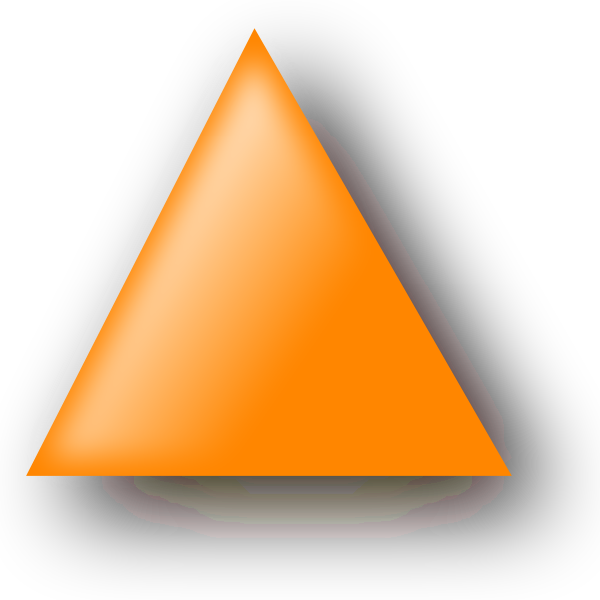
\includegraphics[width=4cm]{images/elemental_mat/triangle}
\end{center}
Then the bounds of the integrals are simply: 
\begin{eqnarray}
\iint_\triangle f(x,y) dx dy &=& 2S \int_0^{1} \left(\int_0^{1-r} f(x(r,s),y(r,s))  ds \right) dr 
\end{eqnarray}
and the mass matrix is given by
\begin{eqnarray}
{\bm M}_e 
&=& 2S \int_{0}^1 \left[ \int_{0}^{1-r}
\left(
\begin{array}{ccc}
(1-r-s)^2 & (1-r-s)r & (1-r-s)s \\
(1-r-s)r & r^2 & rs \\
(1-r-s)s & rs & s^2 
\end{array}
\right)
 ds \right] dr \\
&=& 
2S \int_{0}^1 
\left(
\begin{array}{ccc}
\int_0^{1-r} (1-r-s)^2 ds &\int_0^{1-r} (1-r-s)r ds& \int_0^{1-r} (1-r-s)s ds \\ \\
\int_0^{1-r} (1-r-s)r ds  &\int_0^{1-r} r^2 ds     & \int_0^{1-r} rs ds \\ \\
\int_0^{1-r} (1-r-s)s ds  &\int_0^{1-r} rs ds      & \int_0^{1-r} s^2 ds
\end{array}
\right)
 dr \\
&=& 
2S
\left(
\begin{array}{ccc}
1/12 & 1/24 & 1/24 \\
1/24 & 1/12 & 1/24 \\
1/24 & 1/24 & 1/12
\end{array}
\right)
\\
&=&
\frac{S}{12}
\left(
\begin{array}{ccc}
2 & 1 & 1 \\
1 & 2 & 1 \\
1 & 1 & 2
\end{array}
\right)
\end{eqnarray}
This is Eq.(4.10e) of \textcite{li06}. 
Also note that in the context of the heat transport equation this matrix is multiplied 
by $\rho C_p$ (all under the assumption that these coefficients are constant 
over the whole element).

%We will then compute the ${\bm J}_x$ and ${\bm J}_y$ matrices\footnote{Nobody 
%knows what these matrices are for ... needs to be looked into.}.
The basis functions can also directly be expressed in the $(x,y)$ coordinate system
(see for example Section~\ref{ss:p1}):
\begin{eqnarray}
\bN_1(x,y) &=& \frac{1}{2S} \left( x_2y_3-x_3y_2+(y_2-y_3)x+(x_3-x_2)y   \right) \nn\\
\bN_2(x,y) &=& \frac{1}{2S} \left( x_3y_1-x_1y_3+(y_3-y_1)x+(x_1-x_3)y   \right) \nn\\
\bN_3(x,y) &=& \frac{1}{2S} \left( x_1y_2-x_2y_1+(y_1-y_2)x+(x_2-x_1)y   \right) \nn
\end{eqnarray}
where $S$ is the area of the element.
We then have 
\begin{eqnarray}
\partial_x \bN_1(x,y) &=& \frac{1}{2S}  (y_2-y_3) = \frac{1}{2S} y_{23} \nn\\
\partial_x \bN_2(x,y) &=& \frac{1}{2S}  (y_3-y_1) = \frac{1}{2S} y_{31} \nn\\
\partial_x \bN_3(x,y) &=& \frac{1}{2S}  (y_1-y_2) = \frac{1}{2S} y_{12} \nn\\
\partial_y \bN_1(x,y) &=& \frac{1}{2S}  (x_3-x_2) = \frac{1}{2S} y_{32} \nn\\
\partial_y \bN_2(x,y) &=& \frac{1}{2S}  (x_1-x_3) = \frac{1}{2S} y_{13} \nn\\
\partial_y \bN_3(x,y) &=& \frac{1}{2S}  (x_2-x_1) = \frac{1}{2S} y_{21} \nn
\end{eqnarray}
where we have introduced the notation $x_{ij}=x_i-x_j$ and $y_{ij}=y_i-y_j$.

%We start with
%\begin{eqnarray}
%{\bm J}_x
%&=& \iint_\triangle  \partial_x \vec{\bN}^T \vec{\bN} dV \nn\\
%&=&  \iint_\triangle 
%\left(
%\begin{array}{c}
%\frac{1}{2S}(y_2-y_3) \\
%\frac{1}{2S}(y_3-y_1) \\
%\frac{1}{2S}(y_1-y_2)
%\end{array}
%\right)
%\left(
%\begin{array}{ccc}
%N_1(x,y) & N_2(x,y) & N_3(x,y) 
%\end{array}
%\right) dx dy \nn\\
%&=& \frac{1}{2S} 
%\left(
%\begin{array}{ccc}
%y_{23} \iint_\triangle \bN_1 dx dy & y_{23} \iint_\triangle \bN_2 dx dy & y_{23} \iint_\triangle \bN_3 dx dy \\
%y_{31} \iint_\triangle \bN_1 dx dy & y_{31} \iint_\triangle \bN_2 dx dy & y_{31} \iint_\triangle \bN_3 dx dy \\
%y_{12} \iint_\triangle \bN_1 dx dy & y_{12} \iint_\triangle \bN_2 dx dy & y_{12} \iint_\triangle \bN_3 dx dy 
%\end{array}
%\right) 
%\end{eqnarray}
%We then need to compute
%\begin{eqnarray}
%\iint_\triangle \bN_1(x,y) dx dy 
%&=& 2S \int_0^{1} \left(\int_0^{1-r} \bN_1(x(r,s),y(r,s))  ds \right) dr \nonumber\\ 
%&=& 2S \int_0^{1} \left(\int_0^{1-r} (1-r-s)  ds \right) dr \nonumber\\ 
%&=& 2S \frac{1}{6} \label{eq:elmats:1}\\ 
%\iint_\triangle \bN_2(x,y) dx dy 
%&=& 2S \int_0^{1} \left(\int_0^{1-r} \bN_2(x(r,s),y(r,s))  ds \right) dr \nonumber\\ 
%&=& 2S \int_0^{1} \left(\int_0^{1-r} r  ds \right) dr \nonumber\\ 
%&=& 2S \frac{1}{6} \label{eq:elmats:2}\\ 
%\iint_\triangle \bN_3(x,y) dx dy 
%&=& 2S \int_0^{1} \left(\int_0^{1-r} \bN_3(x(r,s),y(r,s))  ds \right) dr \nonumber\\ 
%&=& 2S \int_0^{1} \left(\int_0^{1-r} s  ds \right) dr \nonumber\\ 
%&=& 2S \frac{1}{6} \label{eq:elmats:3} 
%\end{eqnarray}
%\todo[inline]{verify!! FOR REAL 2025}
%Finally:
%\[
%{\bm J}_x
%=
%\frac{1}{6}
%%\left(
%\begin{array}{ccc}
%y_{23} & y_{23} & y_{23} \\ 
%y_{31} & y_{31} & y_{31} \\ 
%y_{12} & y_{12} & y_{12}  
%\end{array}
%\right) 
%\]
%Likewise
%\begin{eqnarray}
%{\bm J}_y
%&=& \iint_\triangle  \partial_y \vec{\bN}^T \vec{\bN} dV \nn\\
%&=&  \iint_\triangle 
%\left(
%\begin{array}{c}
%\frac{1}{2S}(x_3-x_2) \\
%\frac{1}{2S}(x_1-x_3) \\
%\frac{1}{2S}(x_2-x_1)
%\end{array}
%\right)
%\left(
%\begin{array}{ccc}
%\bN_1(x,y) & \bN_2(x,y) & \bN_3(x,y) 
%\end{array}
%\right) dx dy \nn\\
%&=&
%\frac{1}{6}
%\left(
%\begin{array}{ccc}
%x_{32} & x_{32} & x_{32} \\ 
%x_{13} & x_{13} & x_{13} \\ 
%x_{21} & x_{21} & x_{21}  
%\end{array}
%\right) 
%\end{eqnarray}

We now turn to the advection $\K_a$ and diffusion $\K_d$ matrices.
The gradient matrix ${\bm B}$ is given by 
\[
{\bm B} = 
\left(
\begin{array}{ccc}
\partial_x \bN_1 & \partial_x \bN_2 & \partial_x \bN_3 \\
\partial_y \bN_1 & \partial_y \bN_2 & \partial_y \bN_3 \\
\end{array}
\right)
=
\frac{1}{2S}
\left(
\begin{array}{ccc}
y_{23} & y_{31} & y_{12} \\
x_{32} & x_{13} & x_{21}
\end{array}
\right)
\]
then 
\[
{\bm K}_d 
= \iint_\triangle {\bm B}^T k {\bm B} \; dV
= \iint_\triangle \frac{k}{4S^2}
\left(
\begin{array}{cc}
y_{23} & x_{32} \\ 
y_{31} & x_{13} \\
y_{12} & x_{21}
\end{array}
\right)
\cdot
\left(
\begin{array}{ccc}
y_{23} & y_{31} & y_{12} \\
x_{32} & x_{13} & x_{21}
\end{array}
\right)
\; dV
\]
If the heat conductivity $k$ is constant within the element, then 
the integrand in the expression above is constant with respect to the 
integration and since $\iint_\triangle dV = S$ we then obtain:
\[
{\bm K}_d 
= \frac{k}{4S}
\left(
\begin{array}{cc}
y_{23} & x_{32} \\ 
y_{31} & x_{13} \\
y_{12} & x_{21}
\end{array}
\right)
\cdot
\left(
\begin{array}{ccc}
y_{23} & y_{31} & y_{12} \\
x_{32} & x_{13} & x_{21}
\end{array}
\right)
\]
or
\[
\boxed{
{\bm K}_d 
= \frac{k}{4S}
\left(
\begin{array}{ccc}
y_{23}y_{23} + x_{32}x_{32} & y_{23}y_{31} + x_{32}x_{13} & y_{23}y_{12} + x_{32}x_{21}  \\ 
y_{31}y_{23} + x_{13}x_{32} & y_{31}y_{31} + x_{13}x_{13} & y_{31}y_{12} + x_{13}x_{21}  \\ 
y_{12}y_{23} + x_{21}x_{32} & y_{12}y_{31} + x_{21}x_{13} & y_{12}y_{12} + x_{21}x_{21} 
\end{array}
\right)
}
\]


Turning now to the advection matrix
\begin{eqnarray}
{\bm K}_a 
&=& \iint_\triangle \vec{\bN}^T \vec{\upnu}\cdot {\bm B} \; dV \nn\\
&=& \iint_\triangle \vec{\bN}^T(x,y) \vec{\upnu}(x,y)\cdot {\bm B}(x,y) \; dx dy \nn\\
&=& 2S \iint_\triangle \vec{\bN}^T(x(r,s),y(r,s)) \vec{\upnu}(x(r,s),y(r,s))\cdot {\bm B}(x(r,s),y(r,s)) \; dr ds \nn\\
&=& 2S \iint_\triangle 
\left(
\begin{array}{c} 
1-r-s \\ r \\ s 
\end{array}
\right)
\vec{\upnu}(x(r,s),y(r,s))\cdot 
\frac{1}{2S}
\left(
\begin{array}{ccc}
y_{23} & y_{31} & y_{12} \\
x_{32} & x_{13} & x_{21}
\end{array}
\right)
\; dr ds \nn\\
&=&  \iint_\triangle 
\left(
\begin{array}{c} 
\bN_1(r,s) \\ \bN_2(r,s) \\ \bN_3(r,s)
\end{array}
\right)
\vec{\upnu}(x(r,s),y(r,s))\cdot 
\left(
\begin{array}{ccc}
y_{23} & y_{31} & y_{12} \\
x_{32} & x_{13} & x_{21}
\end{array}
\right)
\; dr ds \nn
\end{eqnarray}
If the velocity is constant within the element (rather rare case) then this can be integrated exactly.
If not, a quadrature rule must be used. 

Let us assume that indeed velocity is constant inside the element. Then 
$\vec{\upnu}(x(r,s),y(r,s))=(u_0,v_0)$ and then
\begin{eqnarray}
{\bm K}_a 
&=&  \iint_\triangle 
\left(
\begin{array}{c} 
\bN_1(r,s) \\ \bN_2(r,s) \\ \bN_3(r,s)
\end{array}
\right)
(u_0,v_0)\cdot 
\left(
\begin{array}{ccc}
y_{23} & y_{31} & y_{12} \\
x_{32} & x_{13} & x_{21}
\end{array}
\right)
\; dr ds \nn \\
&=&  \iint_\triangle 
\left(
\begin{array}{c} 
\bN_1(r,s) \\ \bN_2(r,s) \\ \bN_3(r,s)
\end{array}
\right)
\left(
\begin{array}{ccc}
u_0 y_{23} + v_0 x_{32} &
u_0 y_{31} + v_0 x_{13} &
u_0 y_{12} + v_0 x_{21}
\end{array}
\right)
\; dr ds \nn \\
\end{eqnarray}
Using Eqs.~\eqref{eq:elmats:1},\eqref{eq:elmats:2},\eqref{eq:elmats:3}
we arrive at
\begin{eqnarray}
{\bm K}_a 
&=& 
\frac{S}{3}
\left(
\begin{array}{c} 
1 \\ 1 \\ 1
\end{array}
\right)
\left(
\begin{array}{ccc}
u_0 y_{23} + v_0 x_{32} &
u_0 y_{31} + v_0 x_{13} &
u_0 y_{12} + v_0 x_{21}
\end{array}
\right)
\end{eqnarray}

\todo[inline]{verify!! FOR REAL 2025 probably off by factor S/2 or 2S !!!}














\newpage
\[
{\bm C}_1
=\int_{\partial\Omega_1} \vec{N}^T(x,y) \vec{N}(x,y) d\Gamma
\]
The edge $\partial\Omega_1$ is bounded by the coordinates of nodes $x_1,y_1$
and $x_2,y_2$. This segment can be parameterised by $t\in[0,1]$:
\[
\vec{r}(t) = (1-t)\left(\begin{array}{c} x_1 \\ y_1 \end{array} \right) + 
t \left(\begin{array}{c} x_2 \\ y_2 \end{array} \right)
=
\left(\begin{array}{c} (x_2-x_1)t +x_1 \\ (y_2-y_1)t+y_1 \end{array} \right) 
\]

Let us assume that $C$ is a smooth curve and that it is given by the 
parametric equations $x=h(t)$, $y=g(t)$ and $a\leq t \leq b$. The line integral 
of a function $f(x,y)$ over $C$ is computed as follows. 
\[
\int_C f(x,y) ds = \int_a^b f(h(t),g(t)) \sqrt{\left(\frac{dx}{dt}\right)^2 + \left(\frac{dy}{dt}\right)^2} dt
\]
In our case $dx/dt=x_2-x_1$ and $dy/dt=y_2-y_1$ so 
\[
\sqrt{\left(\frac{dx}{dt}\right)^2 + \left(\frac{dy}{dt}\right)^2}
=\sqrt{(x_2-x_1)^2+(y_2-y_1)^2} = L_1
\]
Then 
\begin{eqnarray}
{\bm C}_1
&=&\int_{\partial\Omega_1} \vec{N}^T(x,y) \vec{N}(x,y) d\Gamma \nn\\
&=&
\left(
\begin{array}{ccc}
\int_{\partial\Omega_1} N_1(x,y)N_1(x,y) d\Gamma & 
\int_{\partial\Omega_1} N_1(x,y)N_2(x,y) d\Gamma &
\int_{\partial\Omega_1} N_1(x,y)N_3(x,y) d\Gamma \\
\int_{\partial\Omega_1} N_2(x,y)N_1(x,y) d\Gamma & 
\int_{\partial\Omega_1} N_2(x,y)N_2(x,y) d\Gamma &
\int_{\partial\Omega_1} N_2(x,y)N_3(x,y) d\Gamma \\
\int_{\partial\Omega_1} N_3(x,y)N_1(x,y) d\Gamma & 
\int_{\partial\Omega_1} N_3(x,y)N_2(x,y) d\Gamma &
\int_{\partial\Omega_1} N_3(x,y)N_3(x,y) d\Gamma 
\end{array}
\right) \nn\\
&=&
L_1
\left(
\begin{array}{ccc}
\int_{0}^1 N_1(x(t),y(t))N_1(x(t),y(t)) dt & 
\int_{0}^1 N_1(x(t),y(t))N_2(x(t),y(t)) dt &
\int_{0}^1 N_1(x(t),y(t))N_3(x(t),y(t)) dt \\\\
\int_{0}^1 N_2(x(t),y(t))N_1(x(t),y(t)) dt & 
\int_{0}^1 N_2(x(t),y(t))N_2(x(t),y(t)) dt &
\int_{0}^1 N_2(x(t),y(t))N_3(x(t),y(t)) dt \\\\
\int_{0}^1 N_3(x(t),y(t))N_1(x(t),y(t)) dt & 
\int_{0}^1 N_3(x(t),y(t))N_2(x(t),y(t)) dt &
\int_{0}^1 N_3(x(t),y(t))N_3(x(t),y(t)) dt
\end{array}
\right) \nn\\
\end{eqnarray}

We are about to compute the individual terms of the matrix
one by one but we will need:
\begin{eqnarray}
S
&=& \frac{1}{2} [(x_1-x_3)(y_2-y_3)-(x_2-x_3)(y_1-y_3)]  \nn\\
&=&  \frac{1}{2} [x_1y_2 -x_1y_3 -x_3y_2 + x_3y_3 -x_2y_1 + x_2y_3 + x_3y_1 - x_3y_3] \nn\\
&=&  \frac{1}{2} [x_1y_2 -x_1y_3 -x_3y_2 -x_2y_1 + x_2y_3 + x_3y_1 ] \nn\\
\end{eqnarray}
and 
\begin{eqnarray}
N_1(x(t),y(t)) 
&=&\frac{1}{2S} [  x_2y_3-x_3y_2+(y_2-y_3)x(t)+(x_3-x_2)y(t) ] \nn\\
&=&\frac{1}{2S} [  x_2y_3-x_3y_2+y_{23}(x_{21} t +x_1)  +x_{32}  (y_{21} t+y_1) ] \nn\\
&=&\frac{1}{2S} [ x_2y_3-x_3y_2 +y_{23}x_1+x_{32}y_1 + (y_{23}x_{21}+x_{32}y_{21}) t  ] \nn\\
&=&\frac{1}{2S} [ \underbrace{x_2y_3-x_3y_2 +x_1y_2-x_1y_3 +x_{3}y_1-x_2y_1}_{2S} \\ 
&& + (x_2y_2-x_1y_2-x_2y_3+x_1y_3 + x_3y_2 - x_3y_1 - x_2y_2 + x_2y_1  ) t  ]  \nn\\
&=&\frac{1}{2S} [ 2S - (\underbrace{x_1y_2+x_2y_3-x_1y_3 - x_3y_2 + x_3y_1 - x_2y_1}_{2S}  ) t  ]  \nn\\
&=&\frac{1}{2S} [ 2S - 2S  t  ] \nn\\
&=&1-t \\
N_2(x(t),y(t)) 
&=& \frac{1}{2S} [ x_3y_1-x_1y_3+(y_3-y_1)(x_{21} t +x_1)+(x_1-x_3)(y_{21} t+y_1)  ] \nn\\
&=& \frac{1}{2S} [ x_3y_1-x_1y_3+(y_3-y_1)x_1+(x_1-x_3)y_1 + (y_{31}x_{21}+x_{13}y_{21}) t ] \nn\\
&=& \frac{1}{2S} [ x_3y_1-x_1y_3+x_1y_3 -x_1y_1+ x_1y_1 -x_3y_1 + (y_{31}x_{21}+x_{13}y_{21}) t ] \nn\\
&=& \frac{1}{2S}   (y_{31}x_{21}+x_{13}y_{21}) t  \nn\\
&=& t \\ 
N_3(x(t),y(t)) 
&=& \frac{1}{2S} ( x_1y_2-x_2y_1+(y_1-y_2)x(t)+(x_2-x_1)y(t)   ) \nn\\
&=& \frac{1}{2S} ( x_1y_2-x_2y_1+(y_1-y_2)( x_{21} t +x_1 )+(x_2-x_1)(y_{21} t+y_1 )   ) \nn\\
&=& \frac{1}{2S} ( x_1y_2-x_2y_1+(y_1-y_2)x_1 +(x_2-x_1)y_1 + (y_{12}x_{21}+x_{21}y_{21})t  ) \nn\\
&=& \frac{1}{2S} ( x_1y_2-x_2y_1+x_1y_1-x_1y_2 +x_2y_1-x_1y_1 + (y_{12}x_{21}-x_{21}y_{12})t     ) \nn\\
&=& 0
\end{eqnarray}


then 

\begin{eqnarray}
\int_{0}^1 N_1(x(t),y(t))N_1(x(t),y(t)) dt 
&=& \int_{0}^1 (1-t)^2 dt = 1/3 \\ 
\int_{0}^1 N_1(x(t),y(t))N_2(x(t),y(t)) dt 
&=& \int_{0}^1 (1-t)t dt = 1/6 \\ 
\int_{0}^1 N_1(x(t),y(t))N_3(x(t),y(t)) dt
&=& 0 \\
\int_{0}^1 N_2(x(t),y(t))N_2(x(t),y(t)) dt 
&=& \int_{0}^1 t^2 dt = 1/3 \\ 
\int_{0}^1 N_2(x(t),y(t))N_3(x(t),y(t)) dt
&=& 0 \\
\int_{0}^1 N_3(x(t),y(t))N_3(x(t),y(t)) dt
&=& 0 
\end{eqnarray}
and finally 
\begin{eqnarray}
{\bm C}_1
&=&\int_{\partial\Omega_1} \vec{N}^T(x,y) \vec{N}(x,y) d\Gamma 
= \frac{L_1}{6}
\left(
\begin{array}{ccc}
2 & 1 & 0 \\
1 & 2 & 0 \\
0 & 0 & 0 
\end{array}
\right) \\
{\bm C}_2 &=&\int_{\partial\Omega_2} \vec{N}^T(x,y) \vec{N}(x,y) d\Gamma 
= \frac{L_2}{6}
\left(
\begin{array}{ccc}
0 & 0 & 0 \\
0 & 2 & 1 \\
0 & 1 & 2 
\end{array}
\right) \\
{\bm C}_3 &=&\int_{\partial\Omega_3} \vec{N}^T(x,y) \vec{N}(x,y) d\Gamma 
= \frac{L_3}{6}
\left(
\begin{array}{ccc}
2 & 0 & 1 \\
0 & 0 & 0 \\
1 & 0 & 2 
\end{array}
\right) 
\end{eqnarray}





